%%%%%%%%%%%%%%%%%%%%%%%%%%%%%%%%%%%%%%%%%%%%%%%%%%%%%%%%%%%%%%%%%%%%%%%%%
%                                                                       %
%              A template file for usage with ustthesis.cls             %
%                                                                       %
%%%%%%%%%%%%%%%%%%%%%%%%%%%%%%%%%%%%%%%%%%%%%%%%%%%%%%%%%%%%%%%%%%%%%%%%%

\documentclass[12pt]{ustthesis}

\usepackage{amsmath, amssymb}
\usepackage{algorithm}
\usepackage{algorithmic}
\usepackage{color,graphicx}
\usepackage{siunitx}
\usepackage{soul}
\usepackage{graphics} % for pdf, bitmapped graphics files
\usepackage{subcaption}
\newtheorem{proof}{Proof}
\usepackage{bookmark}
\usepackage{hyperref} % for better viewing experience  -- added by alan
\usepackage{textcomp}
\usepackage{multirow}
\usepackage{nth}
\usepackage{indentfirst}
\usepackage{siunitx}
\usepackage{changepage}
\usepackage[a4paper, margin=1in]{geometry} % page requriement from the university ---added by Lei.
\usepackage{setspace}
% Alan: begin the font trial
% Euler for math | Palatino for rm | Helvetica for ss | Courier for tt
% \renewcommand{\rmdefault}{ppl} % rm

% NOTE Lei: rouphly 32 lines for 12pt font size and 1.5 line spacing
% \linespread{0.5}
\singlespacing
% \onehalfspacing
%\doublespacing

% \usepackage[scaled]{helvet} % ss
% \usepackage{courier} % tt
% \usepackage{euler} % math
% \usepackage{eulervm} % a better implementation of the euler package (not in gwTeX)
% \normalfont
% \usepackage[T1]{fontenc}
% Alan: end the font trial


\DeclareMathOperator*{\argmax}{\arg\!\max}
\DeclareMathOperator*{\argmin}{\arg\!\min}

\newcommand{\red}[1]{#1}
\newcommand{\tab}[1]{\hspace{3mm}}

% NOTE Lei: personal habit for math symbols.
\newcommand{\bx}{\mathbf{x}}
\newcommand{\bX}{\mathbf{X}}
\newcommand{\by}{\mathbf{y}}
\newcommand{\bY}{\mathbf{Y}}
\newcommand{\bD}{\mathbf{D}}
\newcommand{\bE}{\mathbf{E}}
\newcommand{\ba}{\mathbf{a}}
\newcommand{\bs}{\mathbf{s}}
\newcommand{\bn}{\mathbf{n}}
\newcommand{\bI}{\mathbf{I}}
\newcommand{\bsigma}{\mathbf{\sigma}}
\newcommand{\cS}{\mathcal{S}}
\newcommand{\cX}{\mathcal{X}}
\newcommand{\cA}{\mathcal{A}}
\newcommand{\cB}{\mathcal{B}}
\newcommand{\cD}{\mathcal{D}}
\newcommand{\bu}{\mathbf{u}}
\newcommand{\bv}{\mathbf{v}}
\newcommand{\ts}{\textsuperscript}
\newcommand{\etal}{{\em et al.}}
\newcommand{\norm}[1]{\left\lVert#1\right\rVert}
\DeclareMathOperator{\atantwo}{atan2}
\newcommand{\argminE}{\mathop{\mathrm{argmin}}}

\setcounter{tocdepth}{3}
\setcounter{secnumdepth}{3}

% \renewcommand{\familydefault}{\rmdefault}

% \usepackage{latexsym}
    % Use the "latexsym" package when encountering the following error:
    %   ! LaTeX Error: Command \??? not provided in base LaTeX2e.
% \usepackage{epsf}
    % Use the "epsf" package for including EPS files.

%%%%%%%%%%%%%%%%%%%%%%%%%%%%%%%%%%%%%%%%%%%%%%%%%%%%%%%%%%%%%%%%%%%%%%%%%
%                                                                       %
% Preambles. DO NOT ERASE THEM. Change to suite your particular purpose.%
%                                                                       %
%%%%%%%%%%%%%%%%%%%%%%%%%%%%%%%%%%%%%%%%%%%%%%%%%%%%%%%%%%%%%%%%%%%%%%%%%

\title{Vision-Based Localization and Map Update for Long-Term Navigation in Changing Environments}  % Title of the thesis.
\author{Jingwen~YU}     % Author of the thesis.

% NOTE Lei: choose your degree
% \degree{\MPhil}             % Degree for which the thesis is.
% %% or
% \degree{\PhD}              % Degree for which the thesis is.

\department{Electronic and Computer Engineering}       % Department to which the thesis

\advisor{~Prof.~Ming~LIU}     % Supervisor.

% NOTE Lei: Uncomment this line if you have a co-supervisor/co-advisor
% \coadvisor{Prof.~Mazi~Zhang}     % Co Supervisor.

%\depthead{Prof.~Meimei~Han}    % department head.

%\defencedate{2019}{08}{05}      % \defencedate{year}{month}{day}   NOTE Lei: change it to the submission month when you submit your final version.

% NOTE:
%   According to the sample shown in the guidelines, page number is
%   placed below the bottom margin.  However, if the author prefers
%   the page number to be printed above the bottom margin, please
%   activate the following command.
% \PNumberAboveBottomMargin

\graphicspath{{./figure/}}
\begin{document}

%%%%%%%%%%%%%%%%%%%%%%%%%%%%%%%%%%%%%%%%%%%%%%%%%%%%%%%%%%%%%%%%%%%%%%%%%
%                                                                       %
% Now the actual Thesis. The order of output MUST be followed:          %
%                                                                       %
%    1) TITLEPAGE                                                       %
%                                                                       %
% The \maketitle command generates the Title page as well as the        %
% Signature page.                                                       %
%                                                                       %
%%%%%%%%%%%%%%%%%%%%%%%%%%%%%%%%%%%%%%%%%%%%%%%%%%%%%%%%%%%%%%%%%%%%%%%%%
%\maketitle

%%%%%%%%%%%%%%%%%%%%%%%%%%%%%%%%%%%%%%%%%%%%%%%%%%%%%%%%%%%%%%%%%%%%%%%%%
%                                                                       %
%     2) DEDICATION (Optional)                                          %
%                                                                       %
% The \dedication and \enddedication commands are optional. If          %
% specified it generates a page for dedication.                         %
%
%%%%%%%%%%%%%%%%%%%%%%%%%%%%%%%%%%%%%%%%%%%%%%%%%%%%%%%%%%%%%%%%%%%%%%%%%

% \dedication
% This is an optional section.
% \enddedication

%%%%%%%%%%%%%%%%%%%%%%%%%%%%%%%%%%%%%%%%%%%%%%%%%%%%%%%%%%%%%%%%%%%%%%%%%
%                                                                       %
%     3) SIGNATURE                                                      %
%                                                                       %
% \signature and \endsignature defines the                              %
% signature page of the Thesis especially for ece.                      %
%                                                                       %
%%%%%%%%%%%%%%%%%%%%%%%%%%%%%%%%%%%%%%%%%%%%%%%%%%%%%%%%%%%%%%%%%%%%%%%%%

%\input{chapter/signature}
%%%%%%%%%%%%%%%%%%%%%%%%%%%%%%%%%%%%%%%%%%%%%%%%%%%%%%%%%%%%%%%%%%%%%%%%%
%                                                                       %
%     3) ACKNOWLEDGMENTS                                                %
%                                                                       %
% \acknowledgments and \endacknowledgments defines the                  %
% Acknowledgments of the author of the Thesis.                          %
%                                                                       %
%%%%%%%%%%%%%%%%%%%%%%%%%%%%%%%%%%%%%%%%%%%%%%%%%%%%%%%%%%%%%%%%%%%%%%%%%

%\input{chapter/ack}
%%%%%%%%%%%%%%%%%%%%%%%%%%%%%%%%%%%%%%%%%%%%%%%%%%%%%%%%%%%%%%%%%%%%%%%%%
%                                                                       %
%     4) TABLE OF CONTENTS                                              %
%                                                                       %
%%%%%%%%%%%%%%%%%%%%%%%%%%%%%%%%%%%%%%%%%%%%%%%%%%%%%%%%%%%%%%%%%%%%%%%%%

%\tableofcontents

%%%%%%%%%%%%%%%%%%%%%%%%%%%%%%%%%%%%%%%%%%%%%%%%%%%%%%%%%%%%%%%%%%%%%%%%%
%                                                                       %
%     5) LIST OF FIGURES (If Any)                                       %
%                                                                       %
%%%%%%%%%%%%%%%%%%%%%%%%%%%%%%%%%%%%%%%%%%%%%%%%%%%%%%%%%%%%%%%%%%%%%%%%%

%\listoffigures

%%%%%%%%%%%%%%%%%%%%%%%%%%%%%%%%%%%%%%%%%%%%%%%%%%%%%%%%%%%%%%%%%%%%%%%%%
%                                                                       %
%     6) LIST OF TABLES (If Any)
%                                                                       %
%%%%%%%%%%%%%%%%%%%%%%%%%%%%%%%%%%%%%%%%%%%%%%%%%%%%%%%%%%%%%%%%%%%%%%%%%

%\listoftables

%%%%%%%%%%%%%%%%%%%%%%%%%%%%%%%%%%%%%%%%%%%%%%%%%%%%%%%%%%%%%%%%%%%%%%%%%
%                                                                       %
%     7) ABSTRACT                                                       %
%                                                                       %
% \abstract and \endabstract are used to define a short Abstract for    %
% the Thesis.                                                           %
%                                                                       %
%%%%%%%%%%%%%%%%%%%%%%%%%%%%%%%%%%%%%%%%%%%%%%%%%%%%%%%%%%%%%%%%%%%%%%%%%

\begin{abstract}
For autonomous robot navigation, vision-based system can be easily deployed with 
inexpensive commercial cameras, especially for monocular visual navigation system. 
However, visual sensors are sensitive to environmental changes caused by lighting, object movement, weathers and seasons.
For both indoor and outdoor autnomous navigation, the changes over time can lead to poor localization
and deterioration in map quality. This may lead to a significant drop on robustness, especially for tasks involving repeated traversals such as autnomous path following, i.e. visual teach and repeat task.
To enable long-term autonomous navigation system, the robustness of the system is a must.
While extensive techniques are proposed to strengthen the robustness of localization
through image retrieval or deep-trained image features that are invariant to appearance changes and viewing angle.
They demonstrate impressive performance on changes caused by lighting condition variantion and seasonal changes, 
while they rarely focus on the changes caused by object movement. This kind of changes are rather typical
in situations such as parking lots, warehouses and offices. The movement can cause not only the appearance change,
but also the infeasibility of the previous paths. In extreme condition, object movement may lead to the
number of features to be insufficient, thus the localization fails.
Besides, localization and mapping are tightly-coupled, however, current researchs lack of an emphasis 
on map managment and update for long-term navigation tasks.
Therefore, this proposal focus on the long-term navigation system enabled by visual sensors and targets on
test and improve the localization robustness under environmental changes aroused by object movements.
Moreover, the corresponding map maintance algorithms aiming at record and update the surrounding changes is 
proposed as an important research direction. With the robustness improvement on localization and
mapping under changing environments, the long-term autnomous navigation tasks e.g. autonomous route following,
should be achieved.
\end{abstract}


%%%%%%%%%%%%%%%%%%%%%%%%%%%%%%%%%%%%%%%%%%%%%%%%%%%%%%%%%%%%%%%%%%%%%%%%%
%                                                                       %
%     8) The Actual Contents                                            %
%                                                                       %
% The command \chapters MUST BE USED to ensure that the entire content  %
% of the Thesis is double-spaced (in version 1.0).                      %
%                                                                       %
% However, in version 2.0, \chapters will be automatically added in     %
% the beginning of the first chapter.                                   %
%                                                                       %
%%%%%%%%%%%%%%%%%%%%%%%%%%%%%%%%%%%%%%%%%%%%%%%%%%%%%%%%%%%%%%%%%%%%%%%%%

%%\chapters         % Not necessary with ustthesis.cls (v2.0).

%%%%%%%%%%%%%%%%%%%%%%%%%%%%%%%%%%%%%%%%%%%%%%%%%%%%%%%%%%%%%%%%%%%%%%%%%
%                                                                       %
% Each chapter is defined via the \chapter command. The usual sectional %
% commands of LaTeX are also available.                                 %
%                                                                       %
%%%%%%%%%%%%%%%%%%%%%%%%%%%%%%%%%%%%%%%%%%%%%%%%%%%%%%%%%%%%%%%%%%%%%%%%%



\input{chapter/s0_introduction}

% NOTE Lei:
%    Normally we don't need PART, but I used it in my thesis.
%\part{From Supervisd Learning to Reinforcment Learning}
%\label{part1}
% \input{chapter/s1_obstacle_avoidance}


% NOTE Lei:
%   this is try to set the conlusion as the same level as the PART in bookmark list. Otherwise, in the bookmark list, chapter conlusion will be under the last PART automatically.
% \bookmarksetup{startatroot}
% \addtocontents{toc}{\bigskip}

\chapter{Proposed Direction}
Based on the above investigations over long-term localization\cite{sarlin2019coarse,paton2016bridging} and mapping\cite{qian2022pocd,schmid2022panoptic} algorithms, the proposed directions lie in following three parts. For current map maintenance systems, accurate 6DoF localization is assumed to be solved and provided as a precondition. Therefore, further tests and research on the localization in dynamic scenes are proposed. Regarding the mapping system, multi-experiences localization (MEL)\cite{paton2016bridging} uses multiple traversals information to continuously build topo-metric maps. It proposed a lifelong learning mapping system without considering the large-scale problem, the map size is not scalable over long-term operation. While POCD\cite{qian2022pocd} maintains the map consistent online without considering that the lighting conditions might be changed significantly. Maintenance of multiple maps of the same scene by typical appearance conditions (e.g. day and night, summer and winter) may improve the robustness of long-term navigation.

\section{Localization in Dynamic Scenes}


\section{Map Update and Management}


\section{Dataset}



\chapter{Preliminary Work}
In this chapter, preliminary works toward the proposed directions have been conducted which also serve as the root of motivation and inspiration.

\section{Localization and Mapping}
In this work, I am trying to build an indoor mapping and localization system for a quadruped robot to enable navigation tasks. For the mapping part, LiDAR odometry and mapping (LOAM, A-LOAM\cite{zhang2014loam}) are used during the localization part. In order to implement obstacle avoidance and path planning, an occupancy map is implemented online. However, when an object exists in an occupancy map for a long time, even after it disappears, the occupancy grid occupied by it won't be released. This is due to its bayesian update nature which brings map update to my attention. Part of the result is shown in Fig\ref{fig:quadruped} and Fig \ref{localizationeva}.
\section{Semantic Segmentation}
In this project, I got hands-on experience in training a semantic segmentation network from scratch and via fine-tuning, which achieves the segmentation tasks on a private and small-scale autonomous driving dataset with self-defined semantic classes. This serves as an evaluation of the state-of-the-art segmentation networks' generalization and domain adaptation abilities. In this project, DeepLabV3\cite{chen2017rethinking}, DeepLabV3+\cite{chen2018encoder}, MobileNetV3\cite{howard2019searching}, and BiSeNetV2\cite{yu2021bisenet} have been tested with results in Fig\ref{cross-evaluation} .
\section{2D Object Detection}
In this project, a relationship-oriented perception pipeline for accomplishing daily manipulation tasks is implemented. 2D object detection and semantic relationship inference are combined and explored to achieve object-level manipulation tasks. This builds up my experience in 2D object detection and inspired me to further research the semantic relationship between objects within a certain scene to construct high-level constraints over the consistency of map semantics. Partial results are shown in Fig\ref{fig:pipeline_relationship}. This work has been accepted by the 2022IEEE/RSJ International Conference on Intelligent Robots and Systems(IROS2022) with more information can be referred to \url{https://www.youtube.com/watch?v=48rpq9SoPYo}.
\section{Visual Place Recognition}
Visual place recognition (VPR) in condition-varying environments is
still an open problem. In this paper\cite{ye2022condition}, we propose to use a convolutional autoencoder (CAE) to tackle this problem. We employ a high-level layer of a pre-trained CNN to generate features and train a CAE to map the features to a low-dimensional space to improve the condition invariance property of the descriptor and reduce its dimension at the same time (detailed approach shown in Fig\ref{fig:approach_VPR}). We verify our method in three challenging datasets involving significant illumination changes, and our method is shown to be superior to the state-of-the-art. The code is publicly available in \url{https://github.com/MedlarTea/CAE-VPR}.
\section{Multi-Sensor Fusion Dataset}
This paper\cite{jiao2022fusionportable} proposes the FusionPortable benchmark, a novel multi-sensor dataset with a diverse set of sequences for mobile robots, shown in Fig . This is a great fit for the collection of real-world long-term datasets mentioned in Section \ref{dataset}. We first advance a portable and versatile multi-sensor suite that offers rich sensory information: 10Hz LiDAR point clouds, 20Hz stereo frame images, high-rate and asynchronous events from stereo event cameras, 200Hz acceleration and angular velocity readings from a tactical grade IMU, and 10Hz GPS signal outdoors. Sensors are already temporally synchronized in hardware. This device is lightweight, self-contained, and has plug-and-play support for mobile robots. Second, we construct a dataset by collecting 18 sequences that cover a variety of environments on the campus by exploiting multiple platforms for data collection. 



% \input{chapter/s6_appendices}
\chapter{List of Figures}

\begin{figure}[!ht]
    \centering
    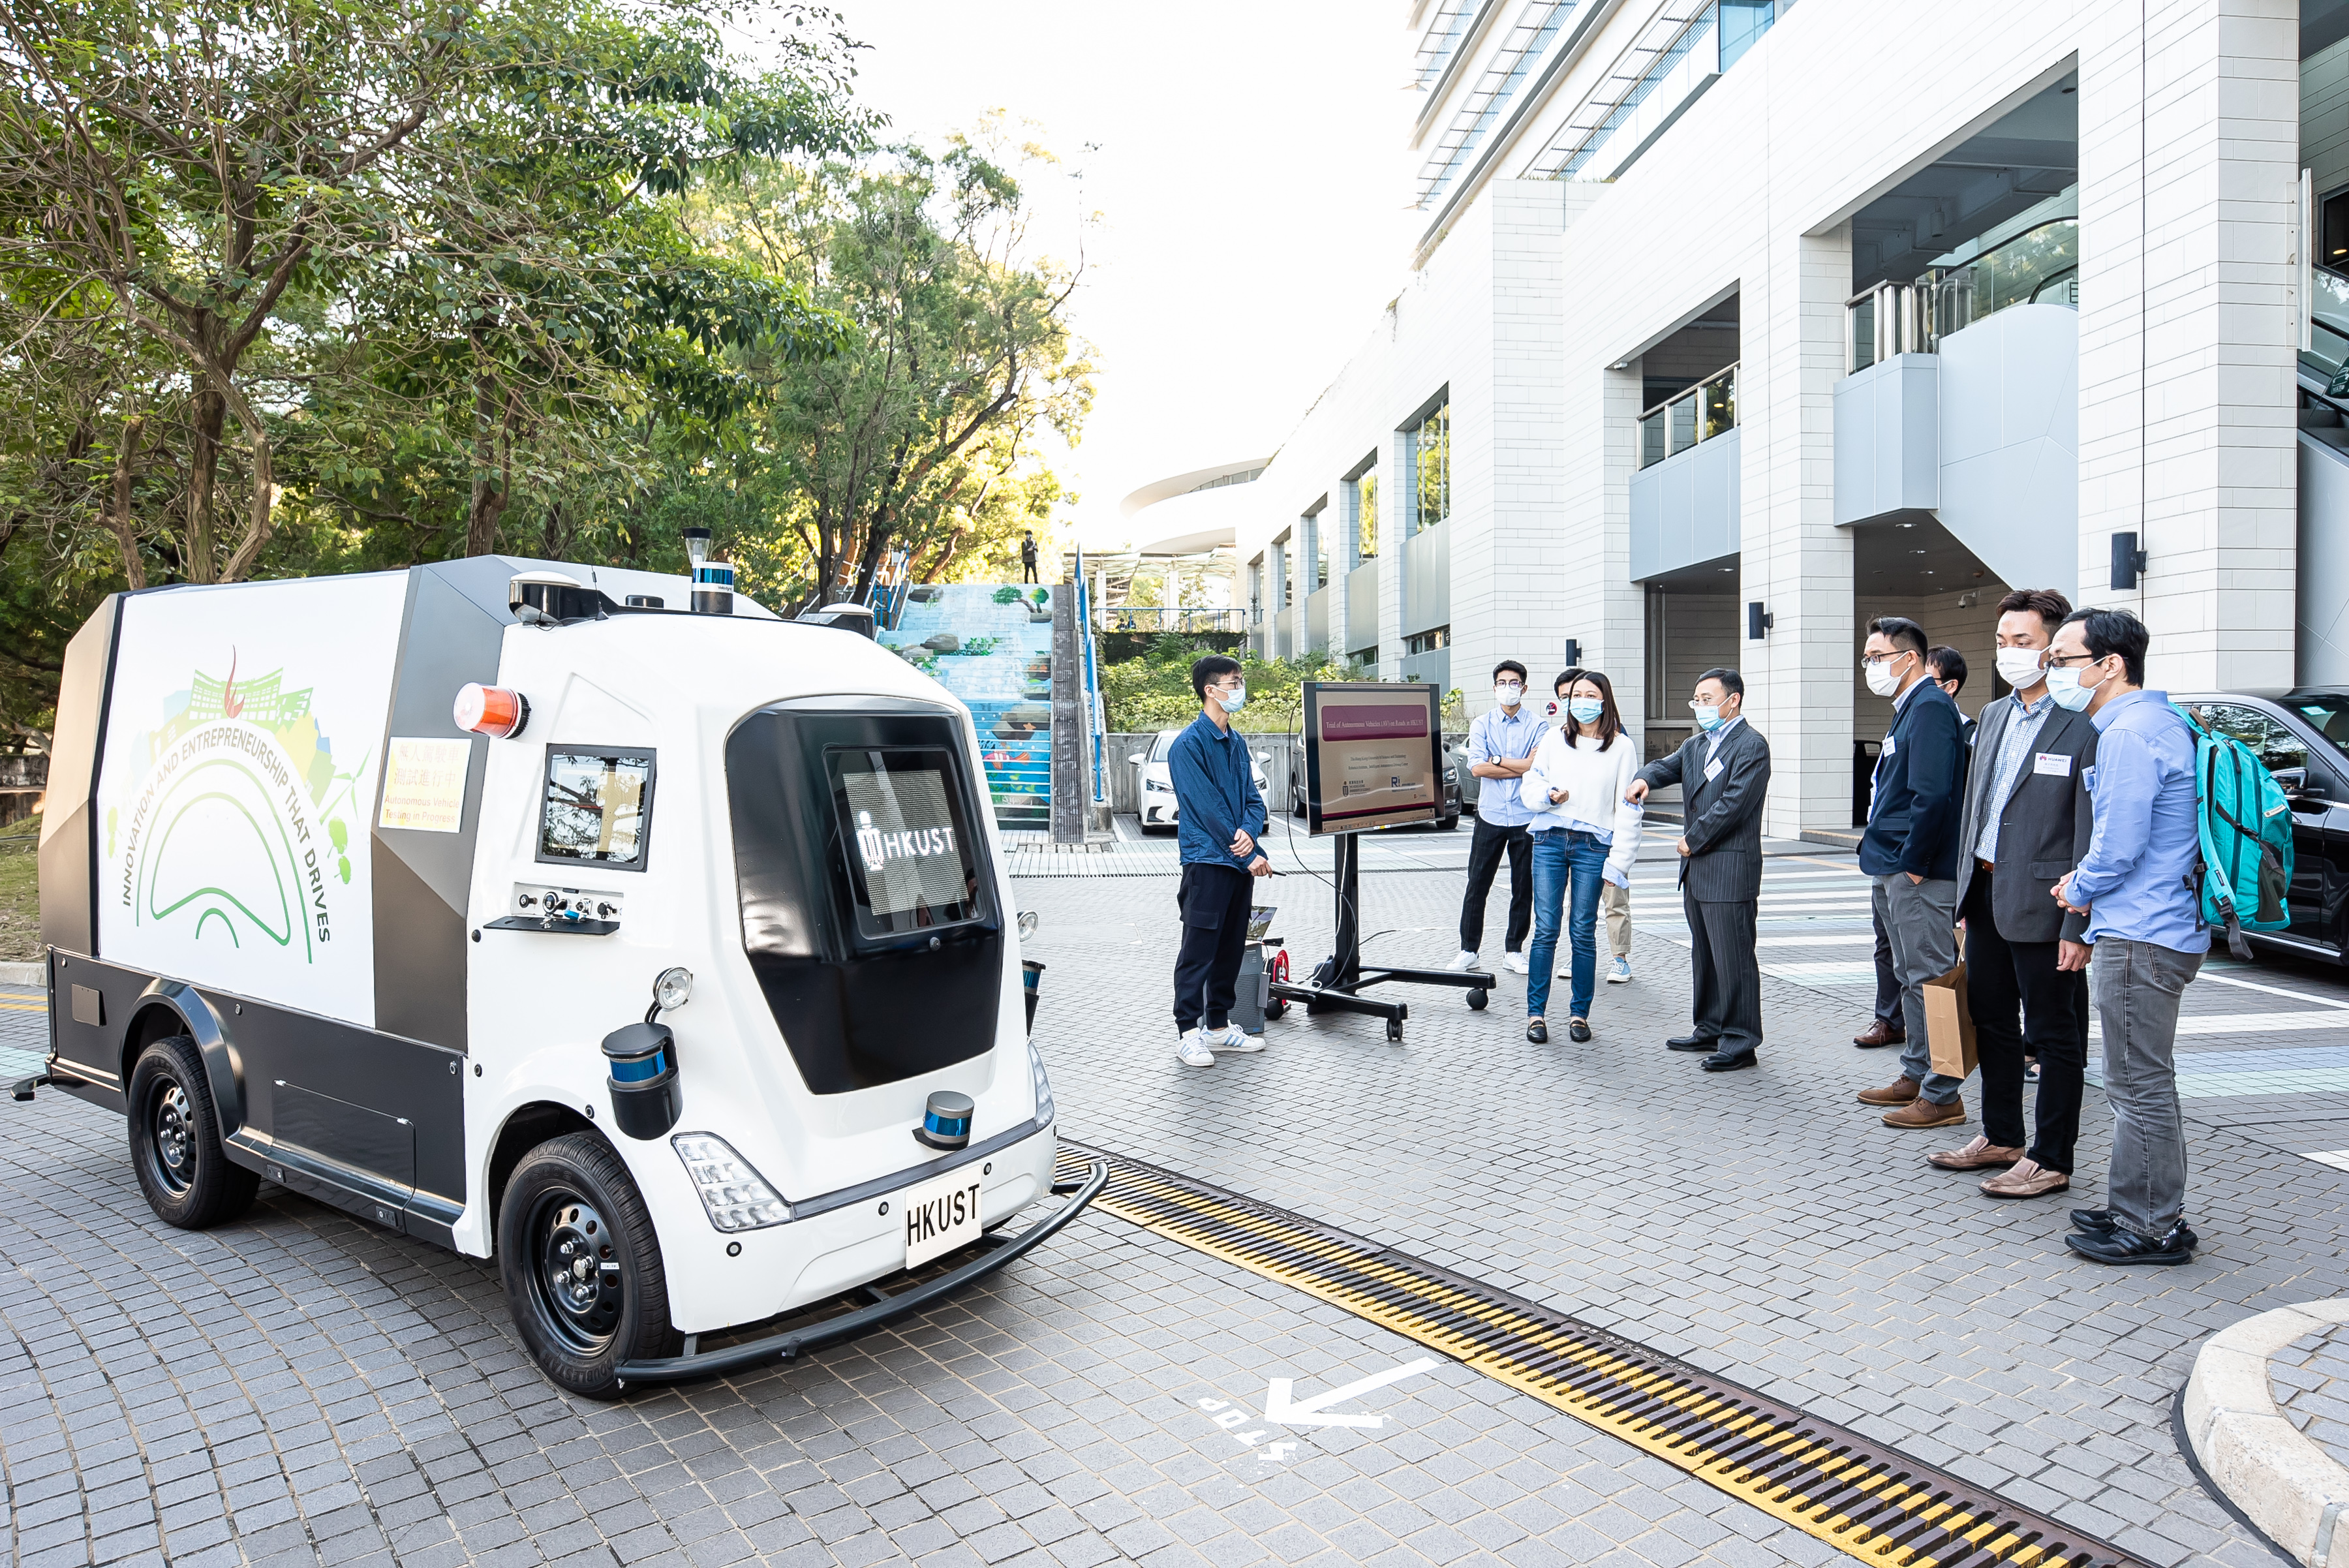
\includegraphics[width=0.9\columnwidth]{figure/pqe/hercules.jpg}
    \caption{The first autonomous vehicle (AV) trial without an operator on board in Hong Kong commenced in late 2020 on the HKUST Clearwater Bay Campus. The AV, designed by Prof. Ming Liu (ECE, Director of HKUST’s Intelligent Autonomous Driving Centre) and his team of students, is one of the many innovative initiatives to fight against the COVID-19 pandemic as the AV can make deliveries that limit human-to-human contact.}
    \label{fig:Hercules}
 \end{figure}

 \begin{figure}[!ht]
    \centering
    \begin{subfigure}{0.45\textwidth}
        \centering
        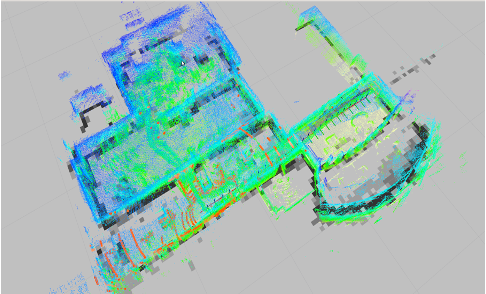
\includegraphics[width=6.5cm, height=4.5cm]{figure/pqe/pointcloudmap.png}
        \caption{A point cloud map of the second floor, HKUST CYT constructed by A-LOAM}
    \end{subfigure}
    \centering
    \begin{subfigure}{0.45\textwidth}
        \centering
        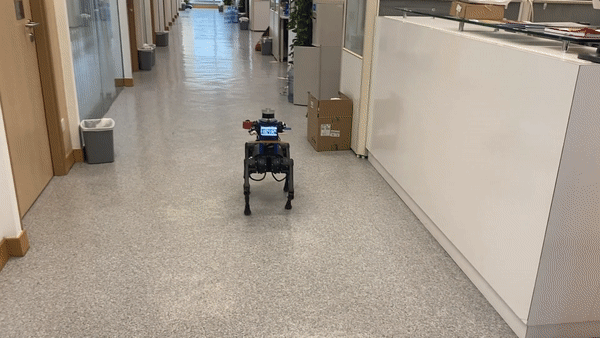
\includegraphics[width=6.5cm, height=4.5cm]{figure/pqe/quadruped.png}
        \caption{A capture of localization on quadruped robot in an indoor office environment.}
    \end{subfigure}
    \caption{Mapping and Localization of Quadruped Robot}
    \label{fig:quadruped}
 \end{figure}

 \begin{figure}[!ht]
    \centering
    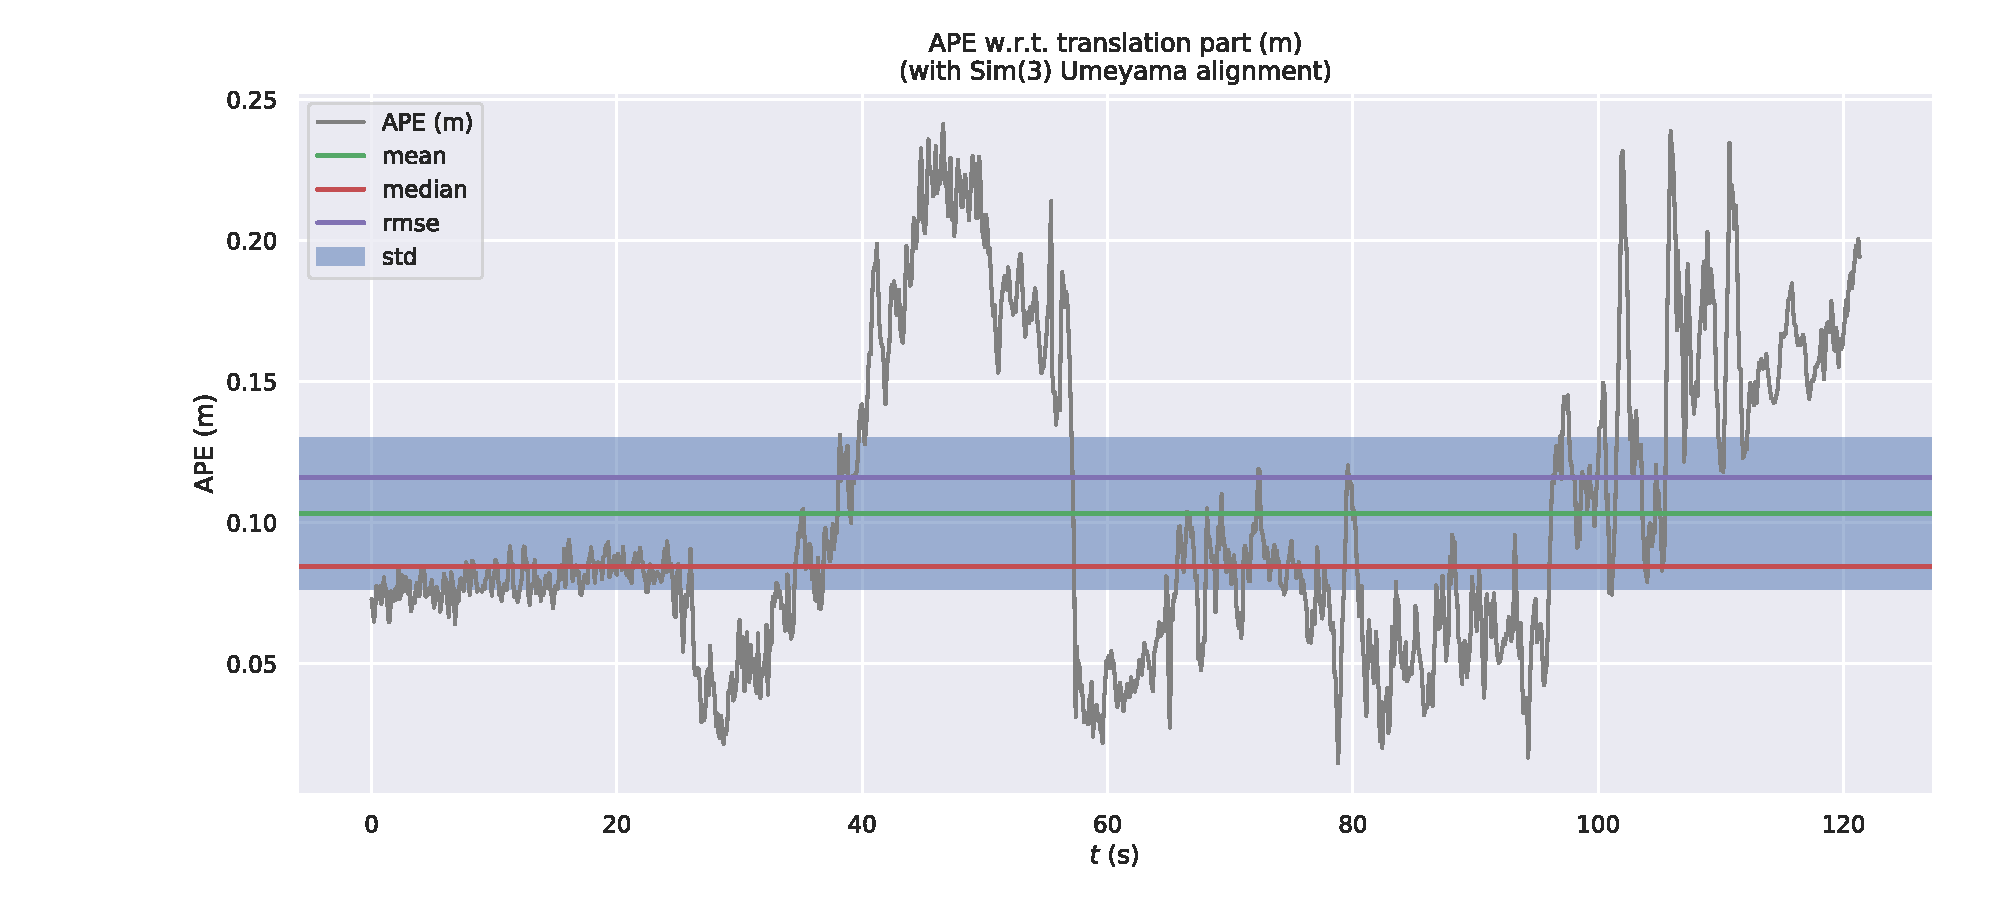
\includegraphics[width=\columnwidth]{figure/pqe/lio2.pdf}
    \caption{Qualitity evaluation result of localization accuracy in the indoor office environment.}
    \label{localizationeva}
 \end{figure}
 \begin{figure}[!ht]
    \centering
    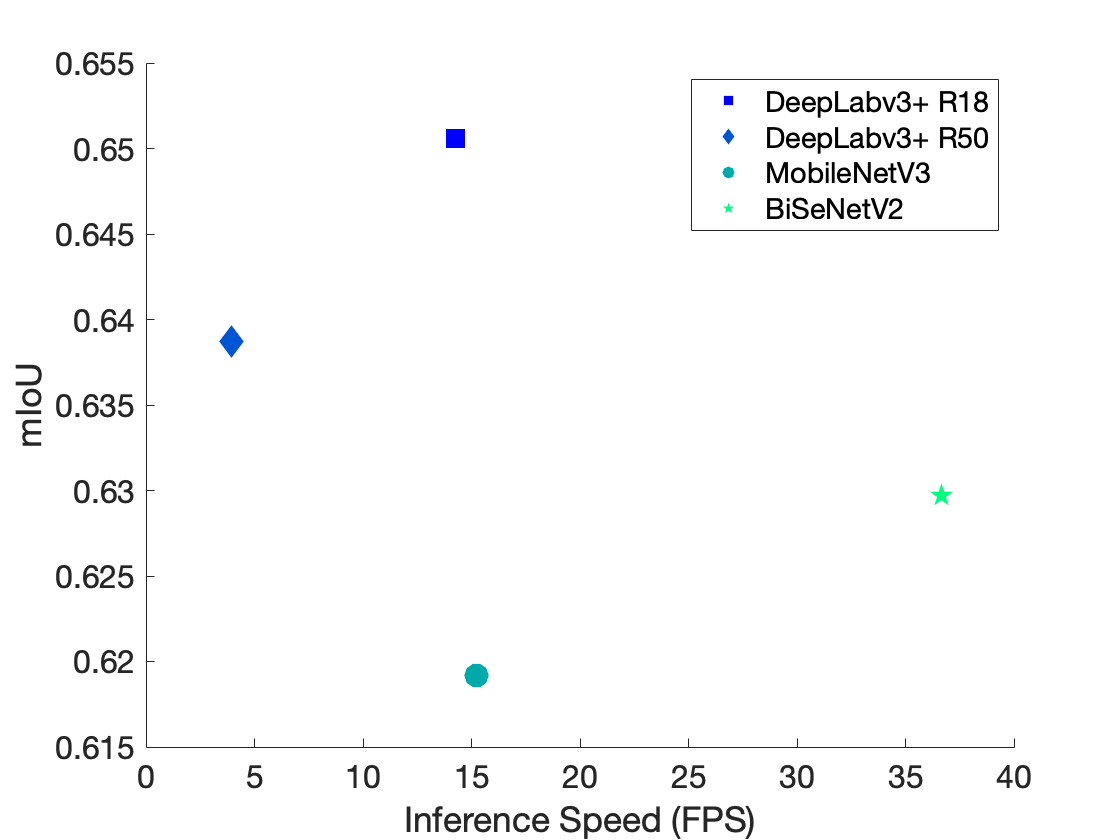
\includegraphics[width=0.75\columnwidth]{figure/pqe/Trade-off.png}
    \caption{The trade-off evaluation between inference speed and segmentation mean Intersection over Union (mIoU) for state-of-the-art segmentation network\cite{yu2021bisenet,howard2019searching,chen2018encoder} }
    \label{cross-evaluation}
 \end{figure}

 \begin{figure}[!ht]
    \centering
    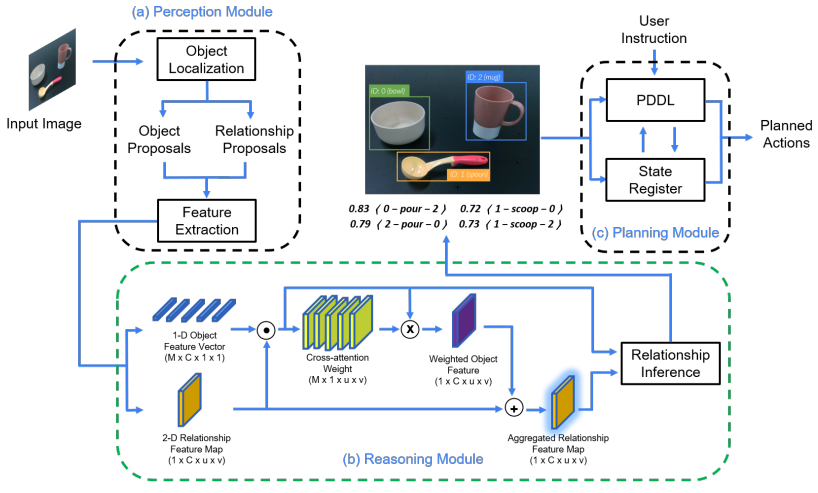
\includegraphics[width=0.9\columnwidth]{figure/pqe/pipeline_relationship.png}
    \caption{The whole pipeline of relationship-oriented semantic scene understanding. Overview: the pipeline first uses (a) perception module to localize all possible object and relationship proposals. A novel relationship-attention
    the mechanism in the (b) reasoning module is then deployed to aggregate the relationship feature map and infer the relationships along with their probabilities.
    Finally, the output from the last step seeds the (c) planning module for goal-oriented, multi-step manipulation task planning according to user instructions. }
    \label{fig:pipeline_relationship}
 \end{figure}

 \begin{figure}[!ht]
    \centering
    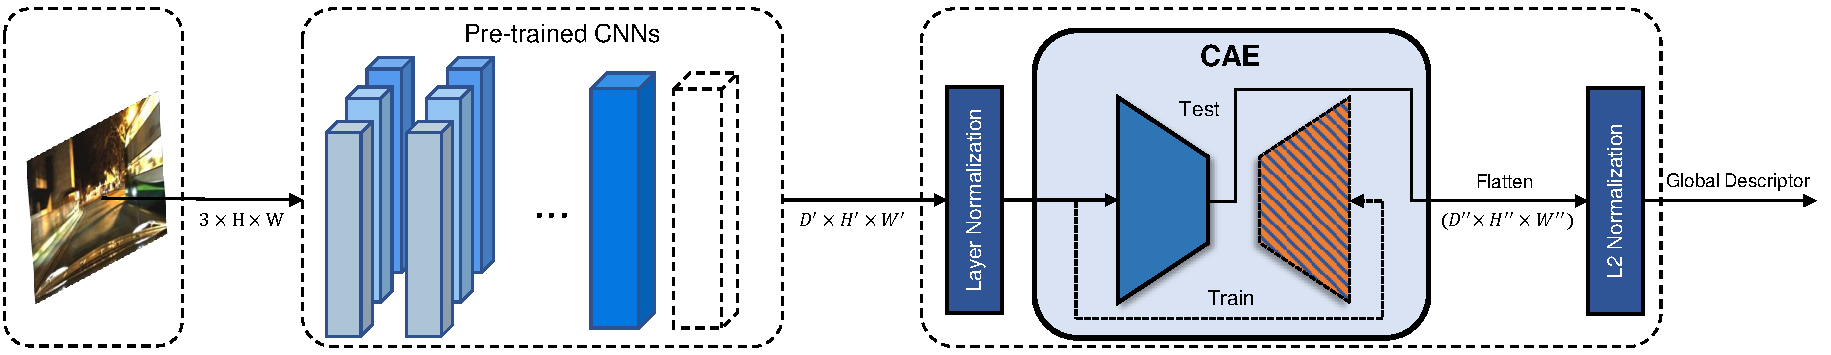
\includegraphics[width=\columnwidth]{figure/pqe/approach.pdf}
	\caption{The detailed pipeline of \cite{ye2022condition}. Given an image with $3\times{H}\times{W}$, CNNs  extract the local feature map $X_i$ with $D^{'}\times{H^{'}}\times{W^{'}}$. The CNNs are classification pre-trained or VPR-trained, e.g. AlexNet, VGG16. Both are cut at the last convolutional layer (conv5), before ReLU. In the training time, CAE is trained unsupervised by a reconstruction loss. In the test time, the decoder part of CAE is not involved and the encoder part is kept to compress the normalized feature map and produce a low-dimensional global descriptor with $D^{''}\times{H^{''}}\times{W^{''}}$. The global descriptor is then flattened and L2 normalized.}
    \label{fig:approach_VPR}
 \end{figure}



\begin{figure}[!ht]
\centering
\begin{subfigure}{0.4\textwidth}
    \centering
    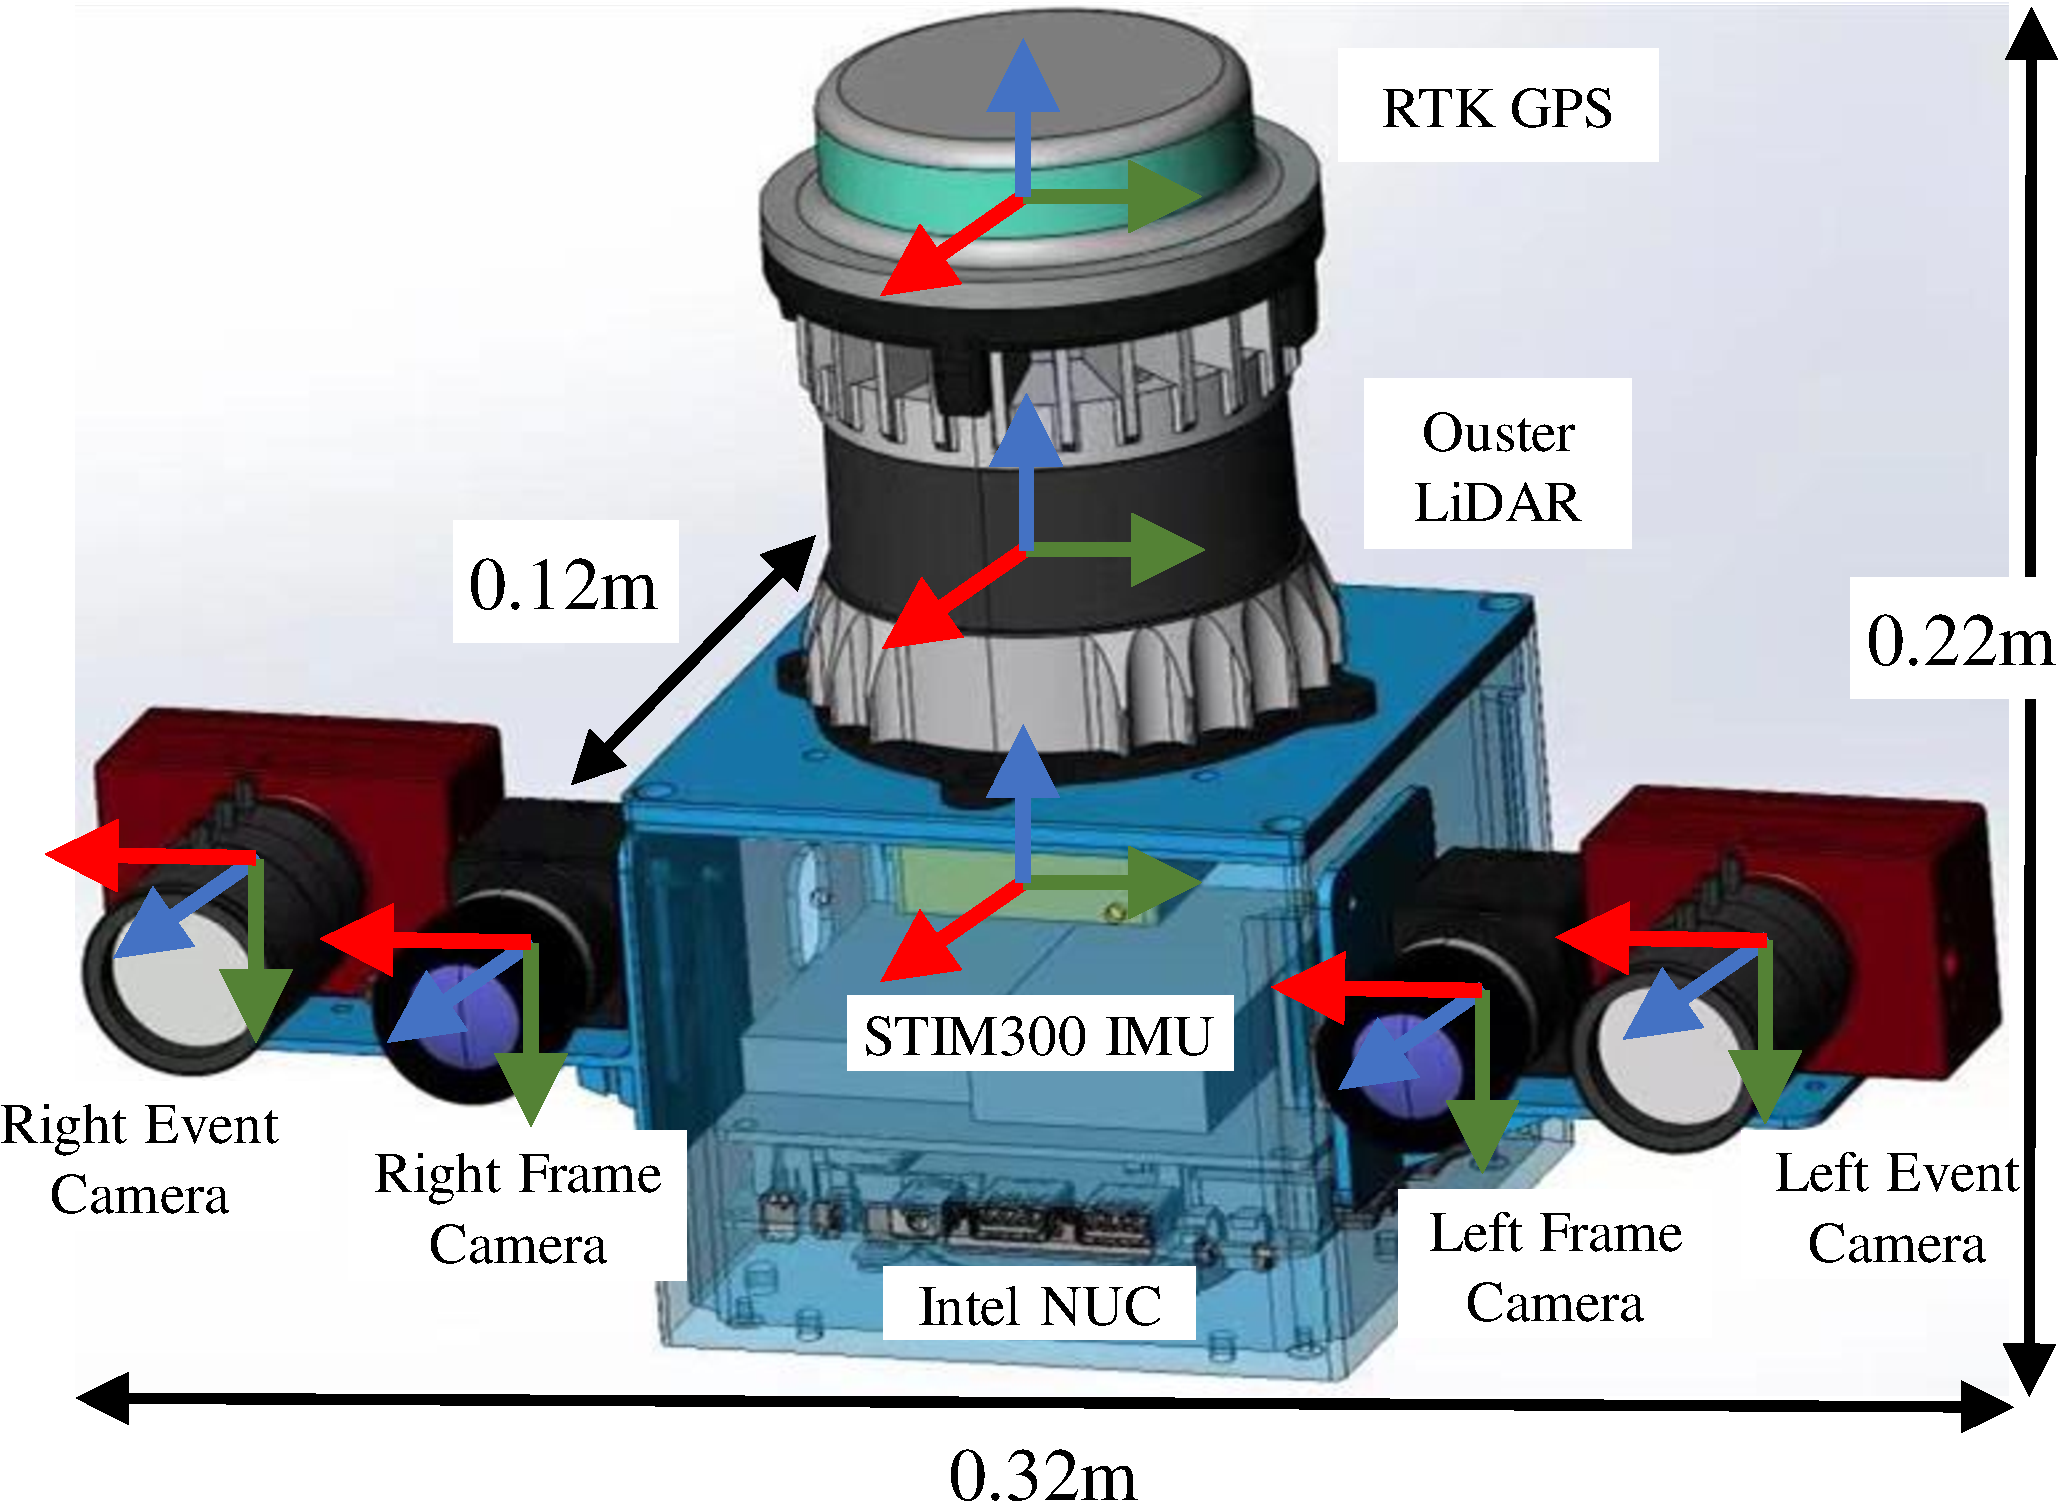
\includegraphics[width=0.8\textwidth, height=5cm]{figure/pqe/methodology/handheld_device-crop.pdf}
    \caption{}
    % \caption{A point cloud map of the second floor, HKUST CYT constructed by A-LOAM}
\end{subfigure}
\centering
\begin{subfigure}{0.4\textwidth}
    \centering
    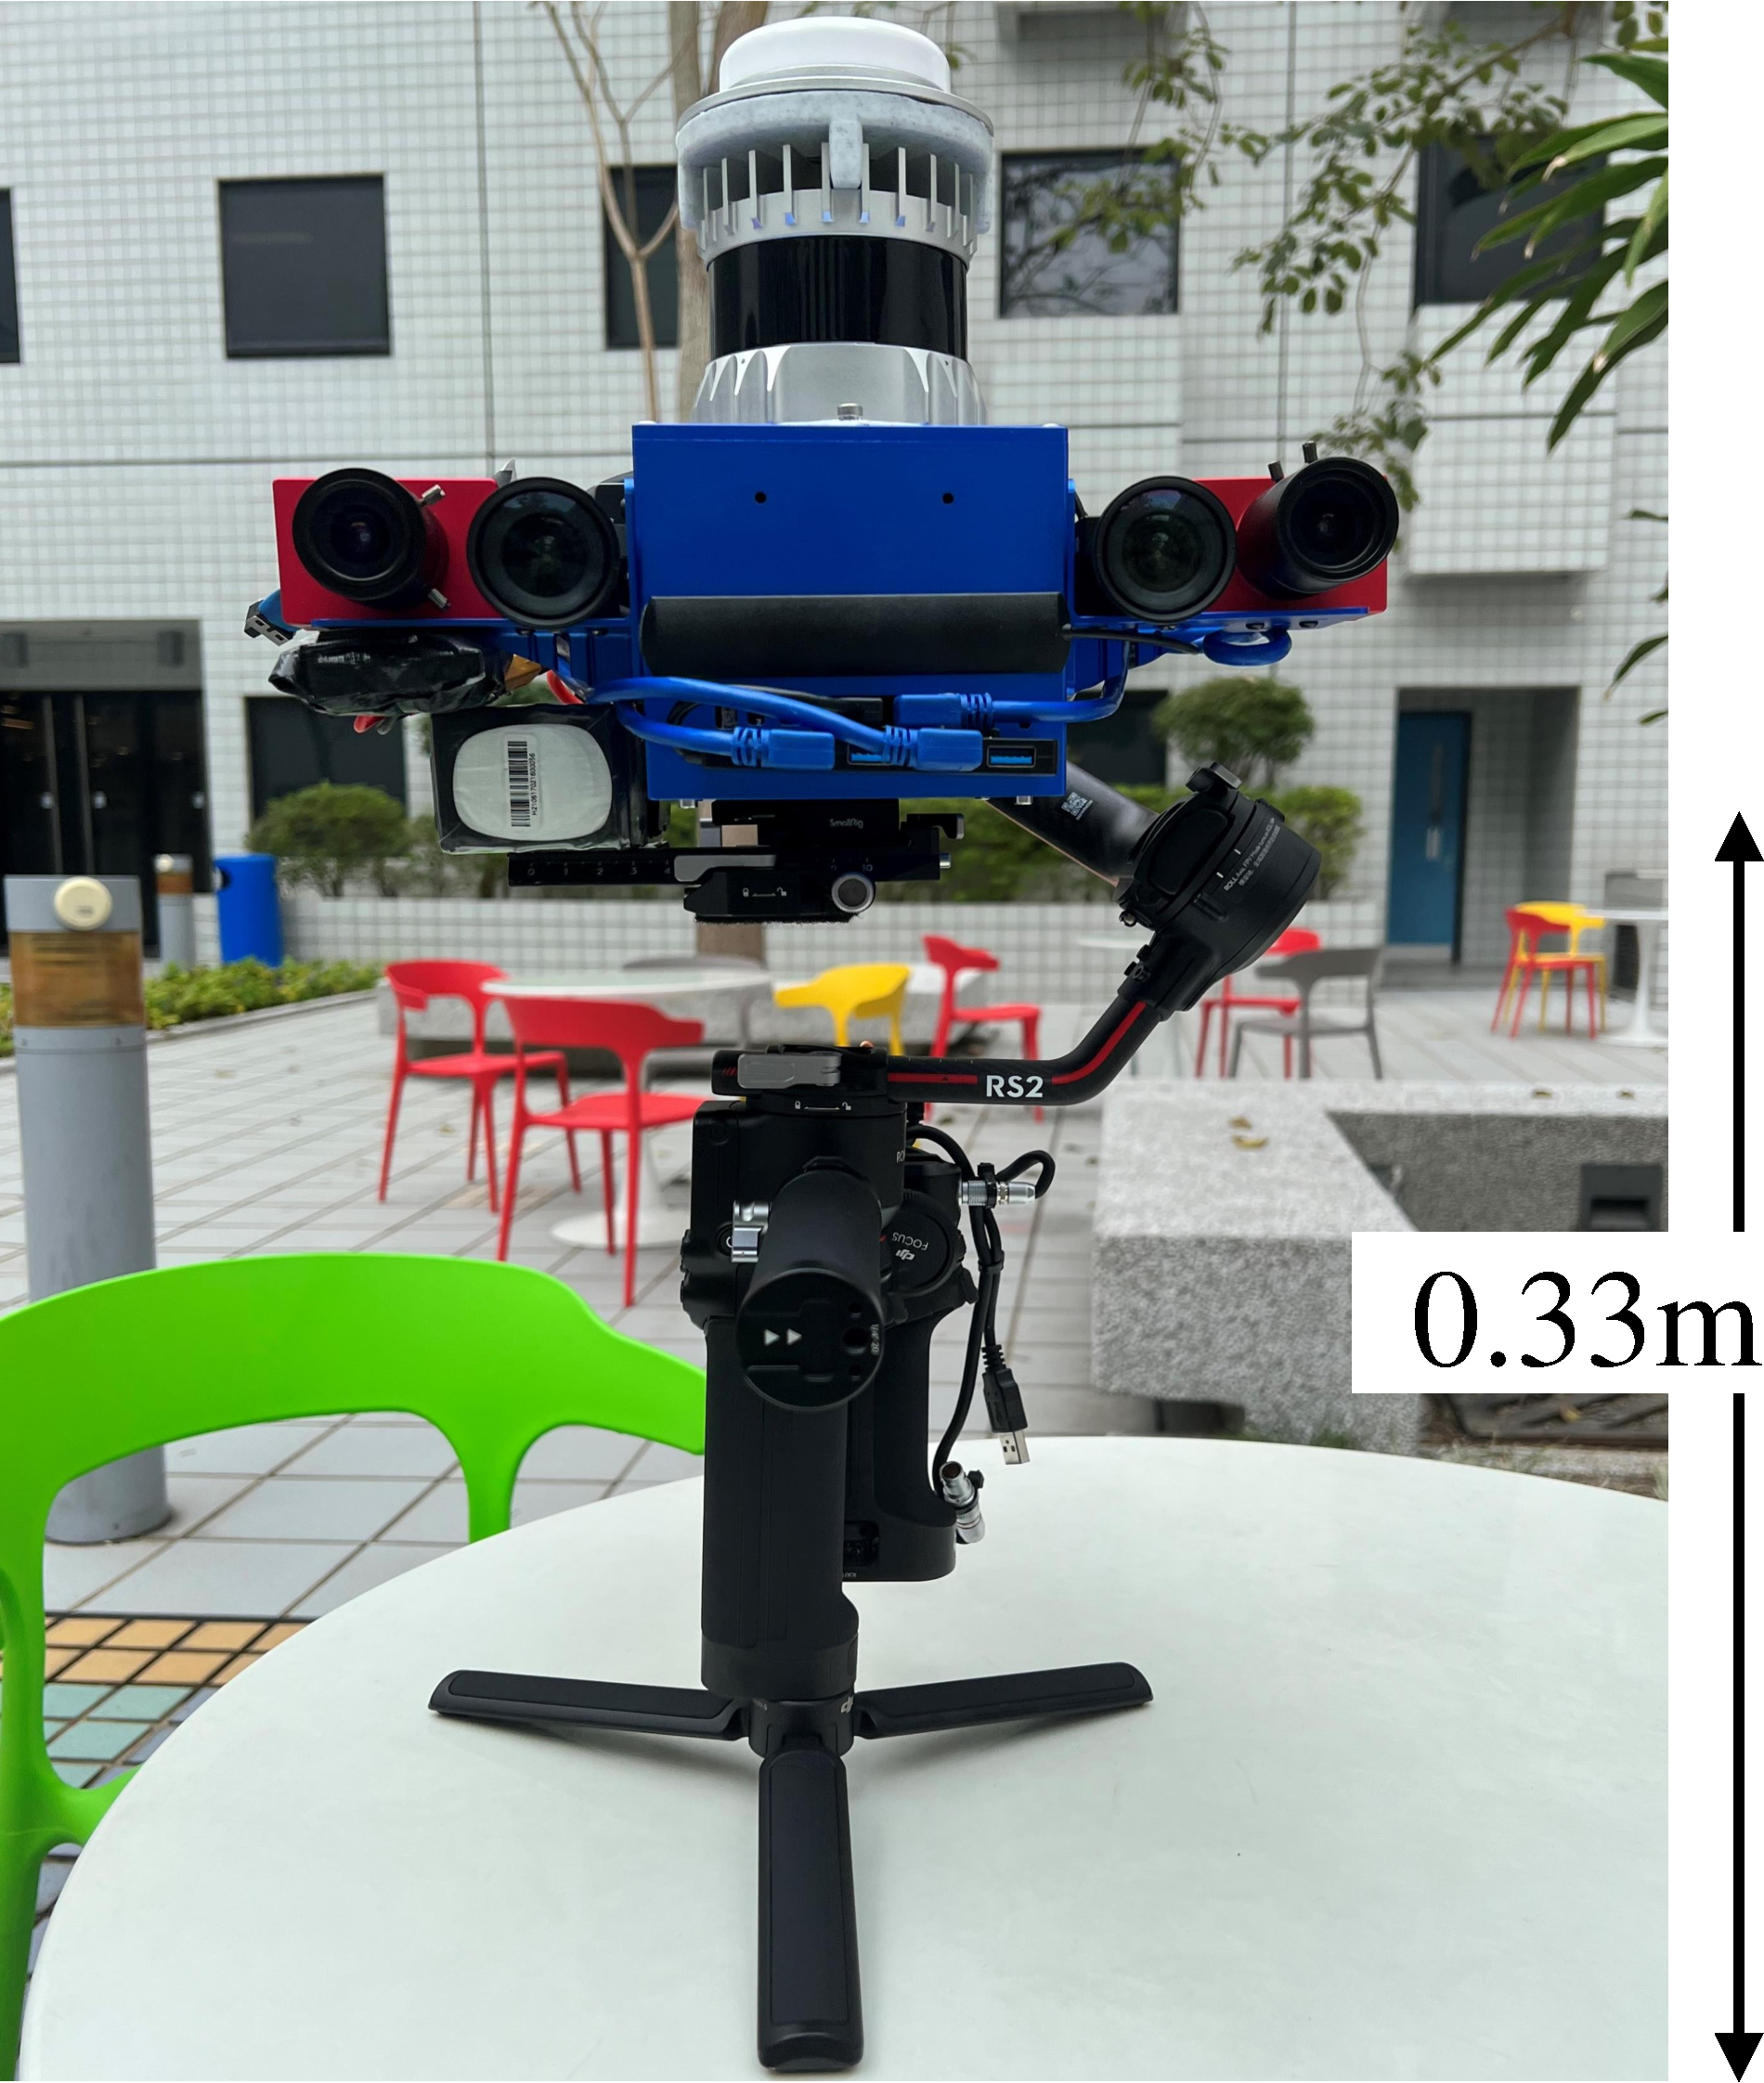
\includegraphics[width=0.8\textwidth, height=5cm]{figure/pqe/methodology/handheld_2-crop.pdf}
    \caption{}
    % \caption{A capture of localization on quadruped robot in an indoor office environment.}
\end{subfigure}
\begin{subfigure}{0.4\textwidth}
    \centering
    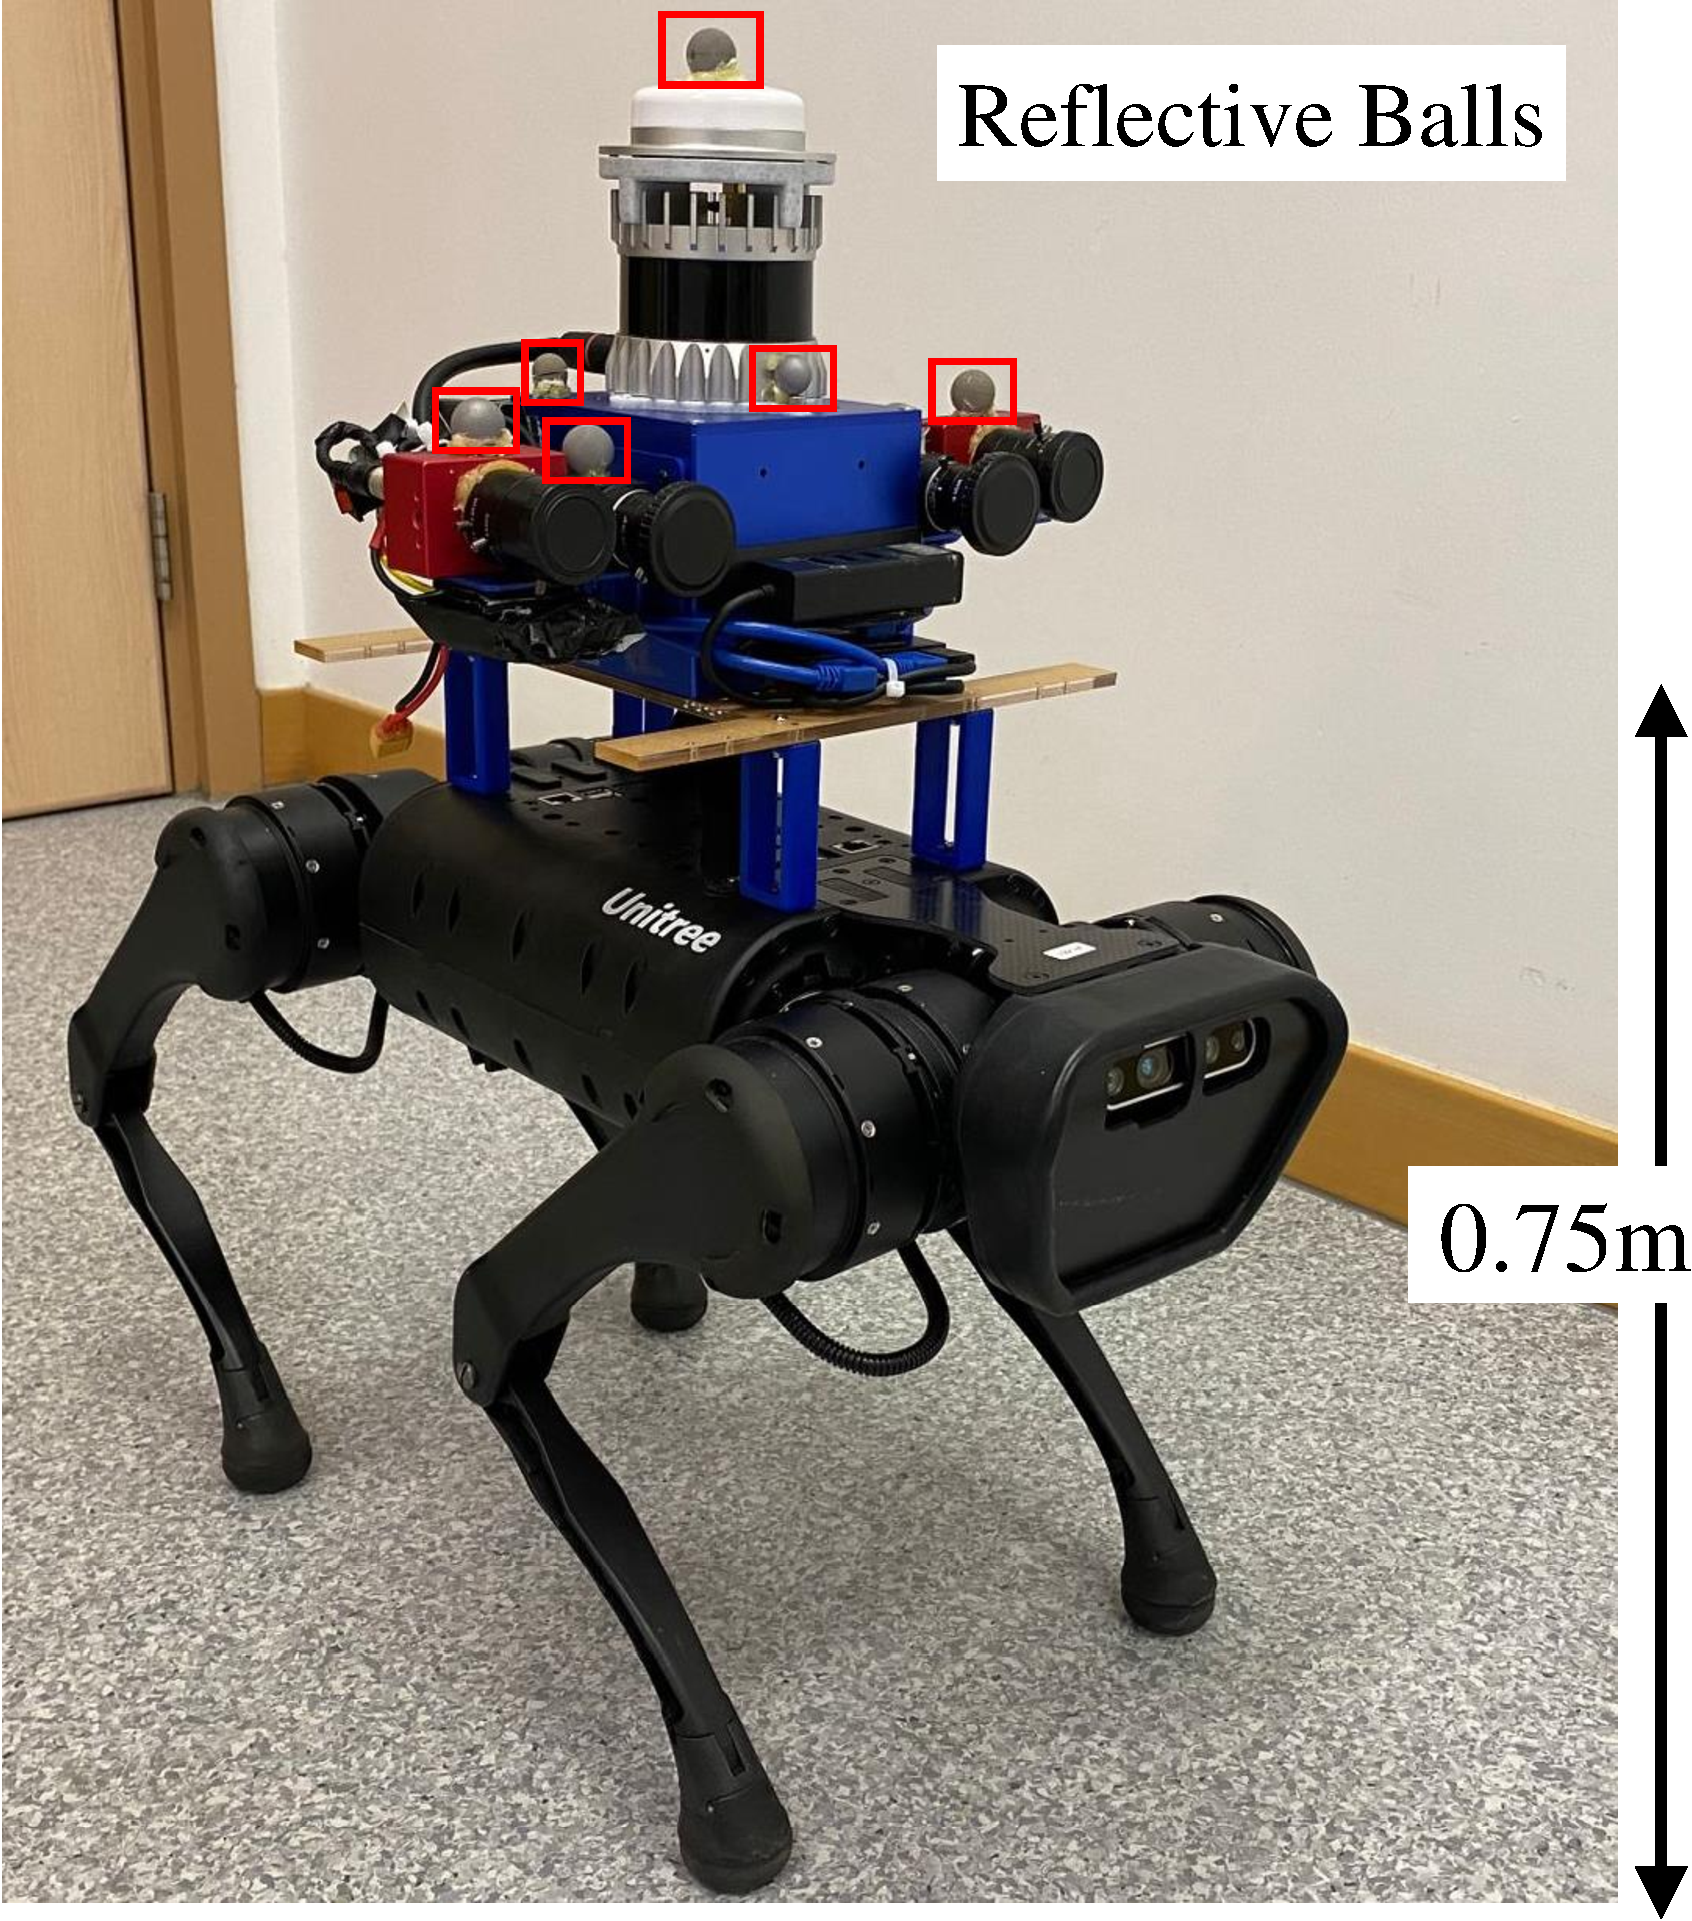
\includegraphics[width=0.8\textwidth, height=5cm]{figure/pqe/methodology/robotdog-crop.pdf}
    \caption{}
    % \caption{A capture of localization on quadruped robot in an indoor office environment.}
\end{subfigure}
\begin{subfigure}{0.4\textwidth}
    \centering
    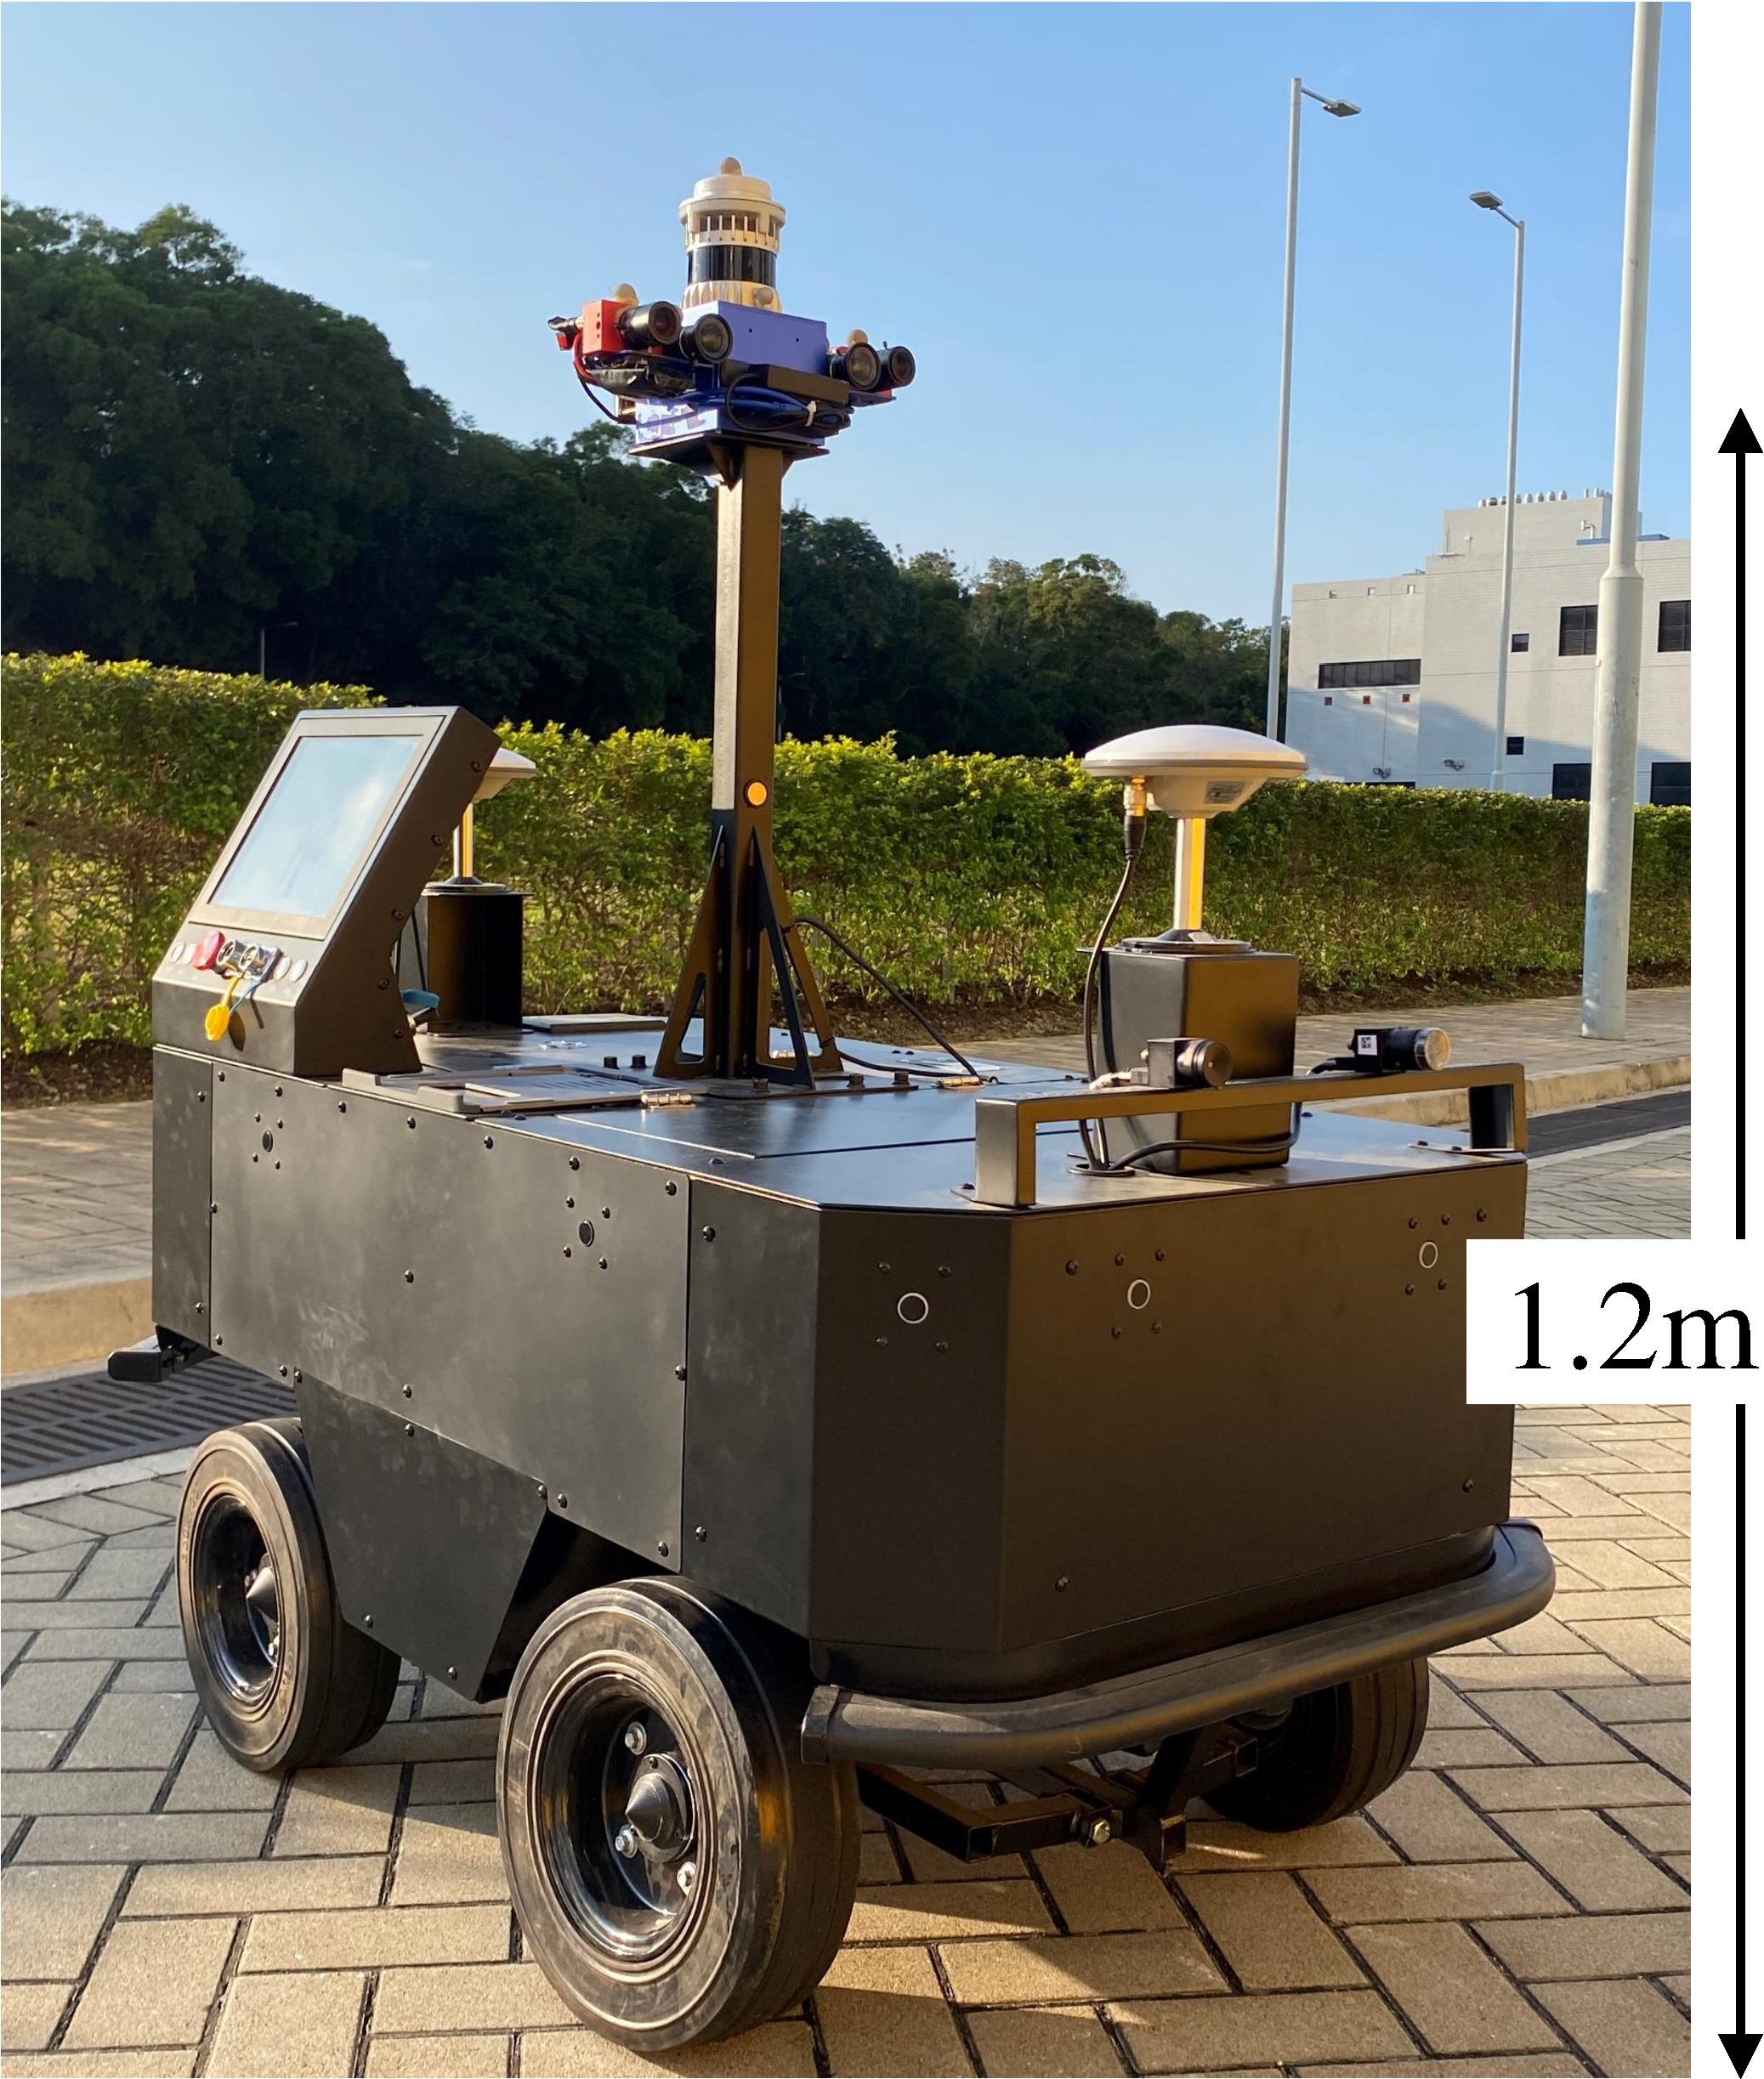
\includegraphics[width=0.8\textwidth, height=5cm]{figure/pqe/methodology/apollo-crop.pdf}
    \caption{}
    % \caption{A capture of localization on quadruped robot in an indoor office environment.}
\end{subfigure}

\caption{The multi-sensor device and data collection platform: 
(a) CAD model of the sensor rig, where axis directions are colored: red: $X$, green: $Y$, blue: $Z$. The sensor rig is rigidly mounted on (b) a gimbal stabilizer, (c) a quadruped robot, and (d) an apollo autonomous vehicle.}
\label{fig:FusionPortable}
\end{figure}
 
 



% \begin{figure}[ht]
% \centering
% \begin{subfigure}
% {\label{fig:sensor_handheld}
% \hspace{0.2cm}
% \centering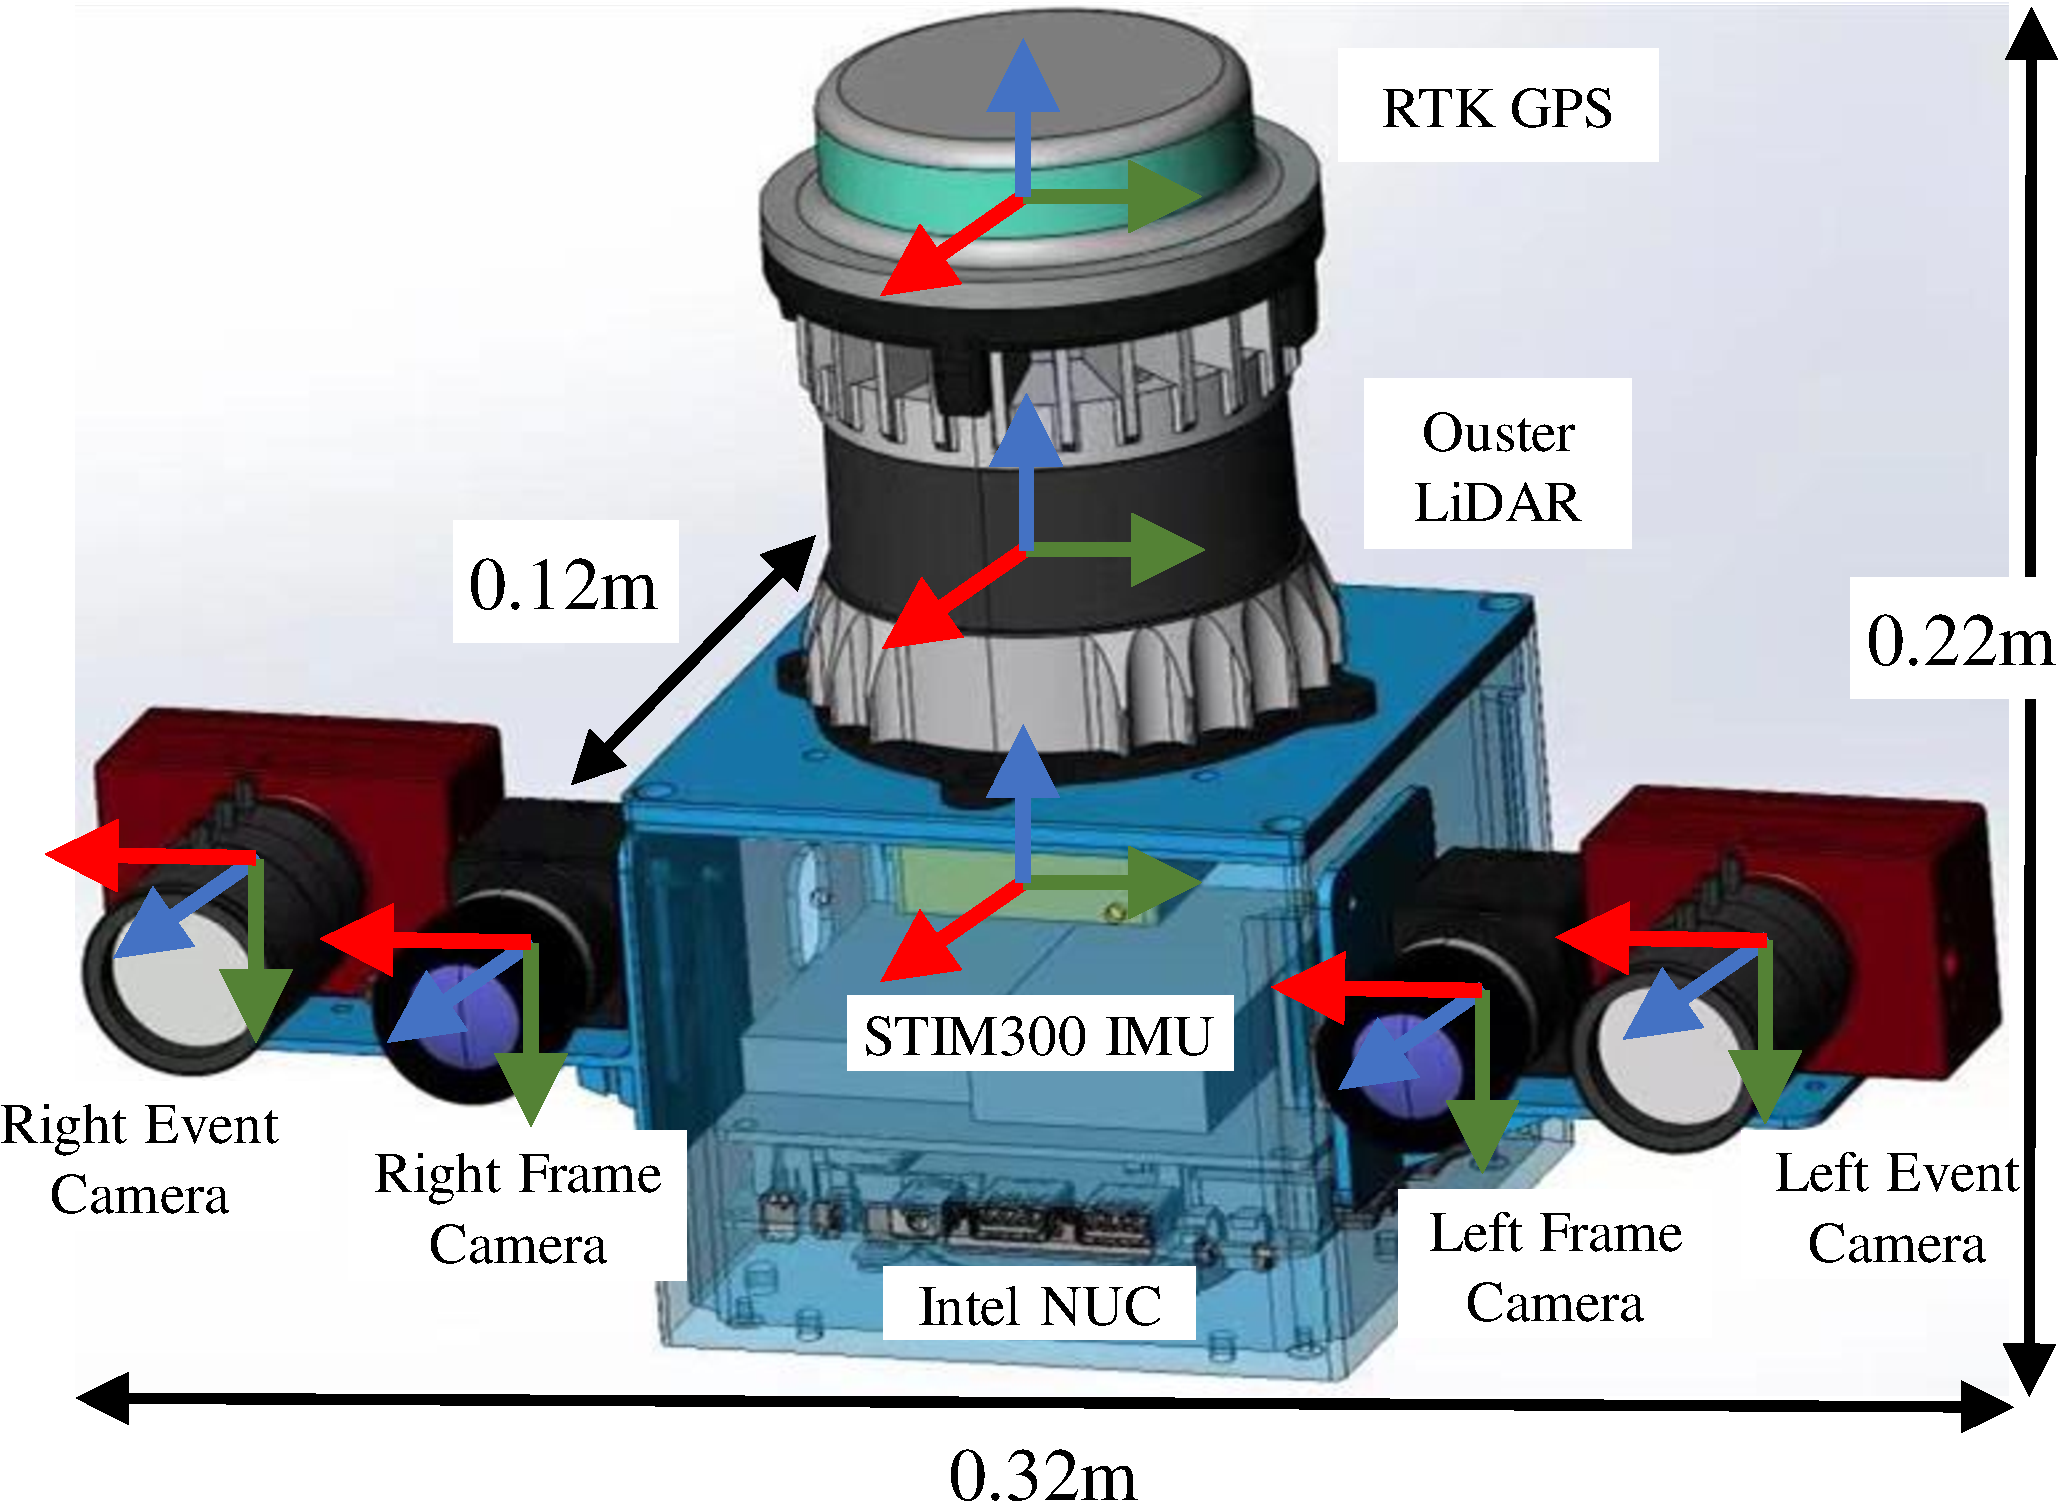
\includegraphics[width=.2746\linewidth]{figure/pqe/methodology/handheld_device-crop.pdf}}
% \end{subfigure}
% \begin{subfigure}{\label{fig:sensor_stab}\centering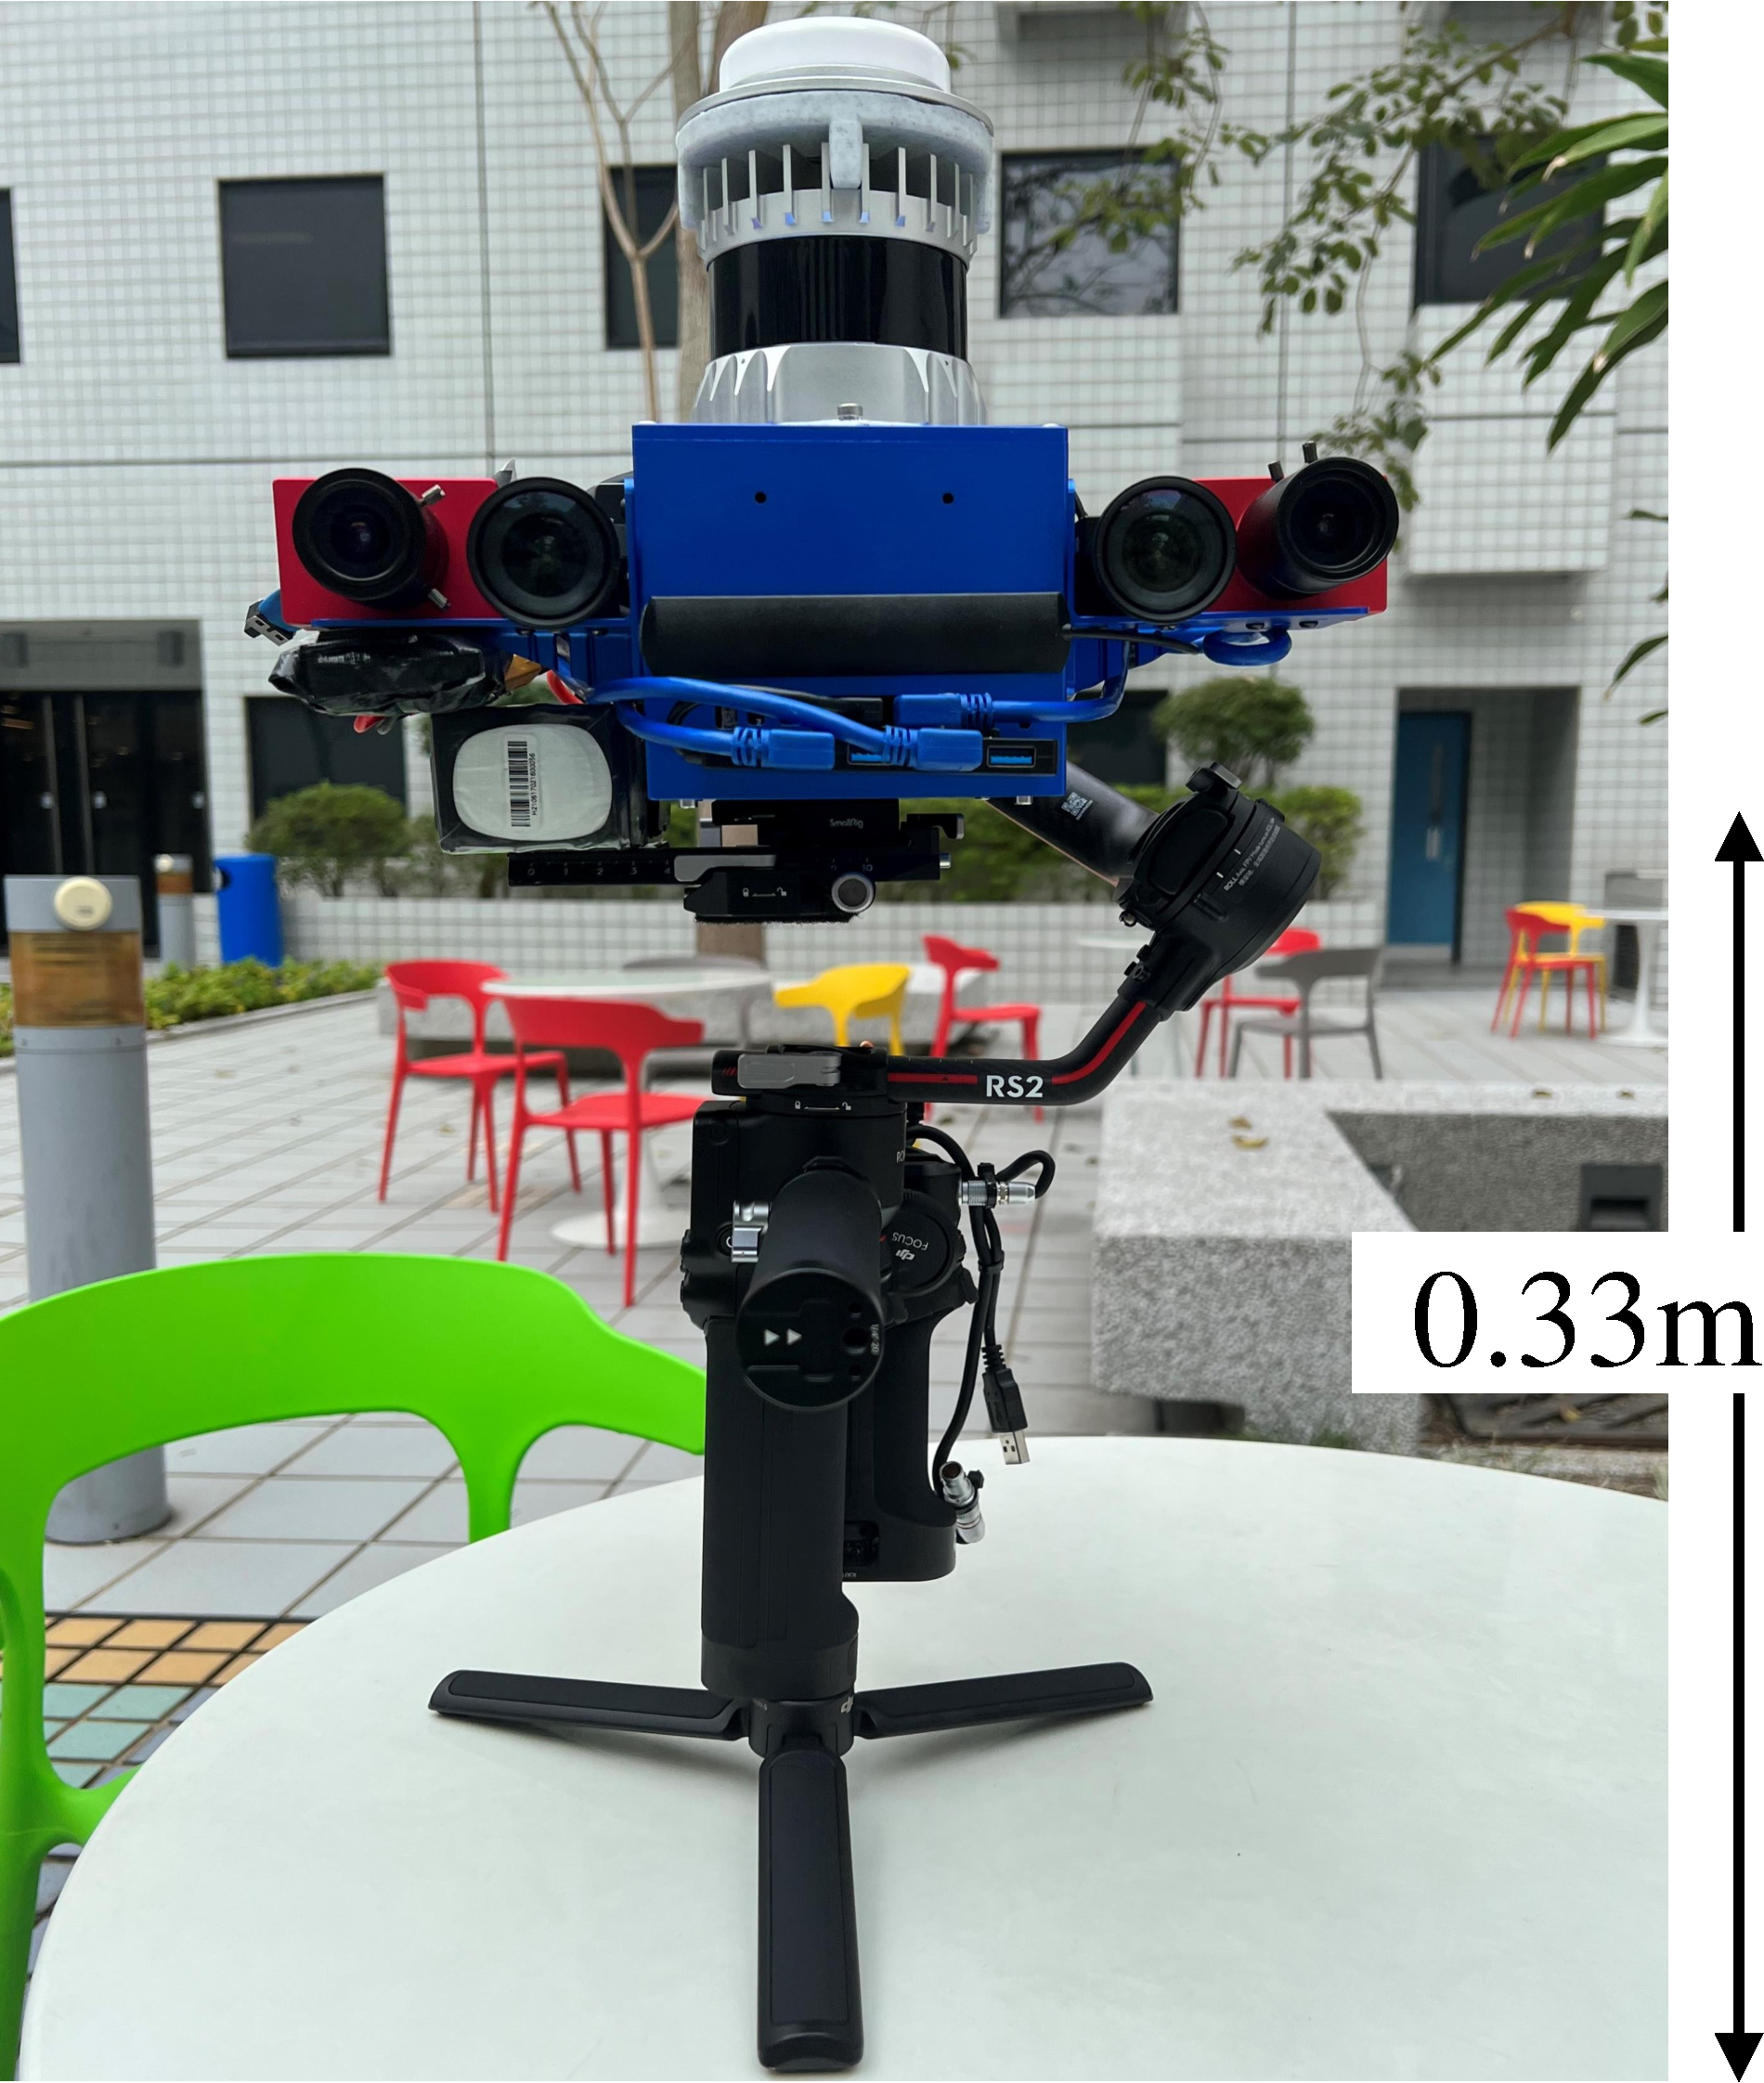
\includegraphics[width=.1701\linewidth]{figure/pqe/methodology/handheld_2-crop.pdf}}
% \end{subfigure}
% \begin{subfigure}{\label{fig:sensor_quadrobot}\centering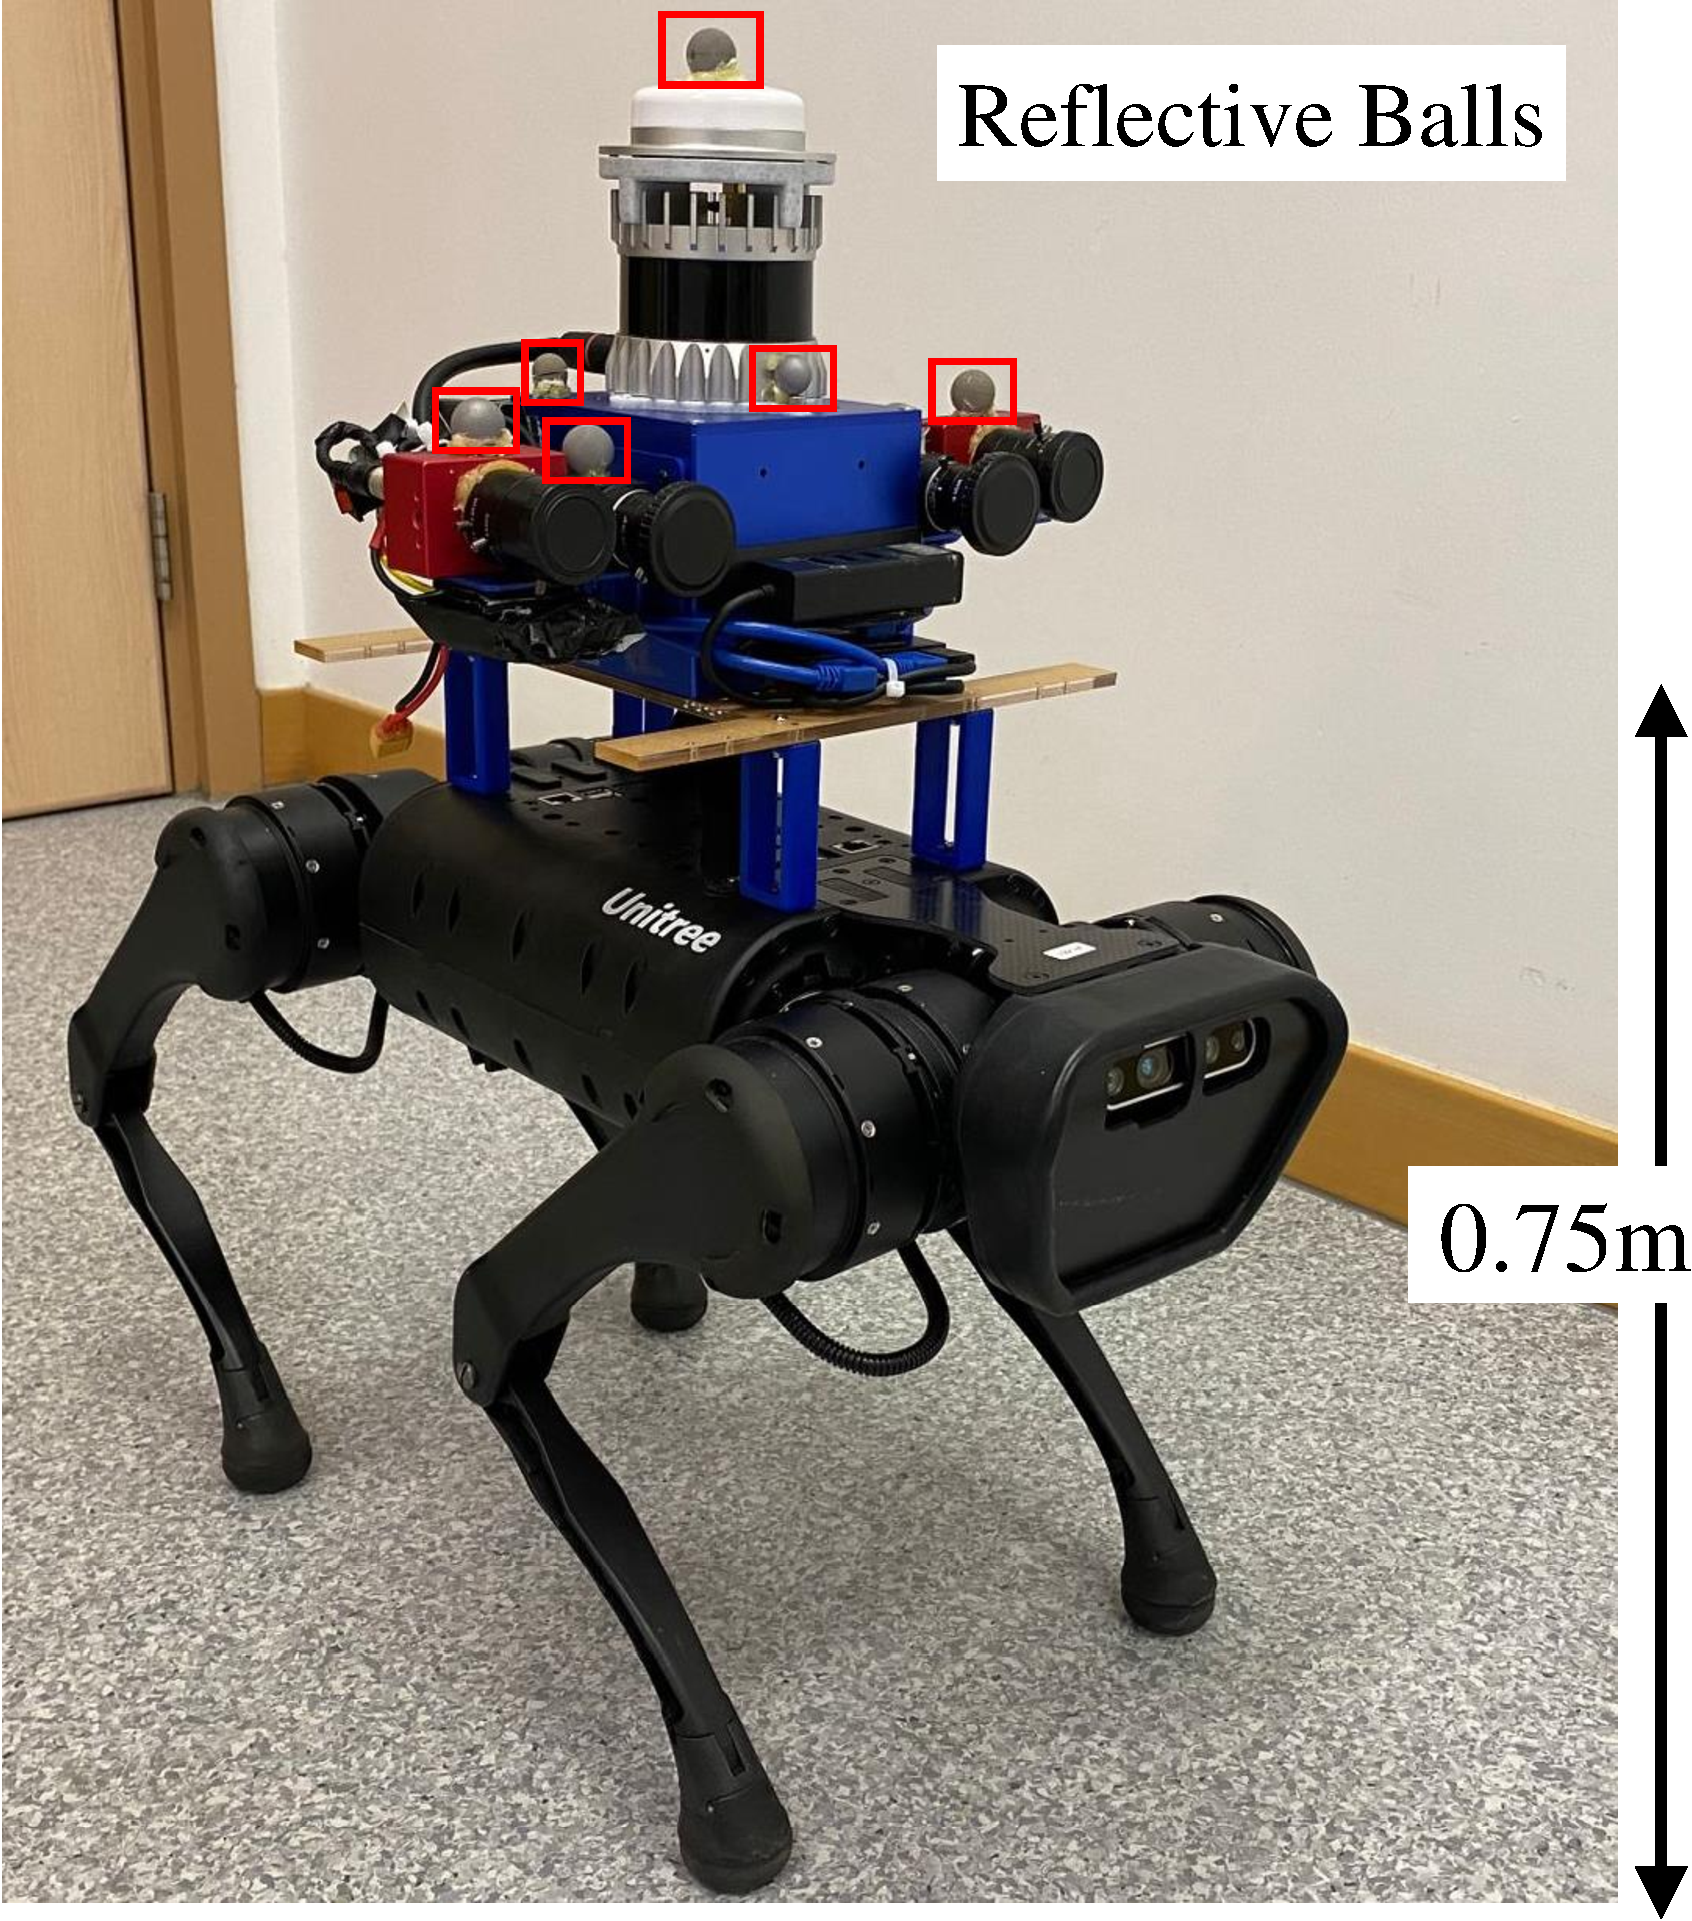
\includegraphics[width=.1776\linewidth]{figure/pqe/methodology/robotdog-crop.pdf}}
% \hspace{0.2cm}
% \end{subfigure}
% \begin{subfigure}
%     {\label{fig:sensor_apollo}\centering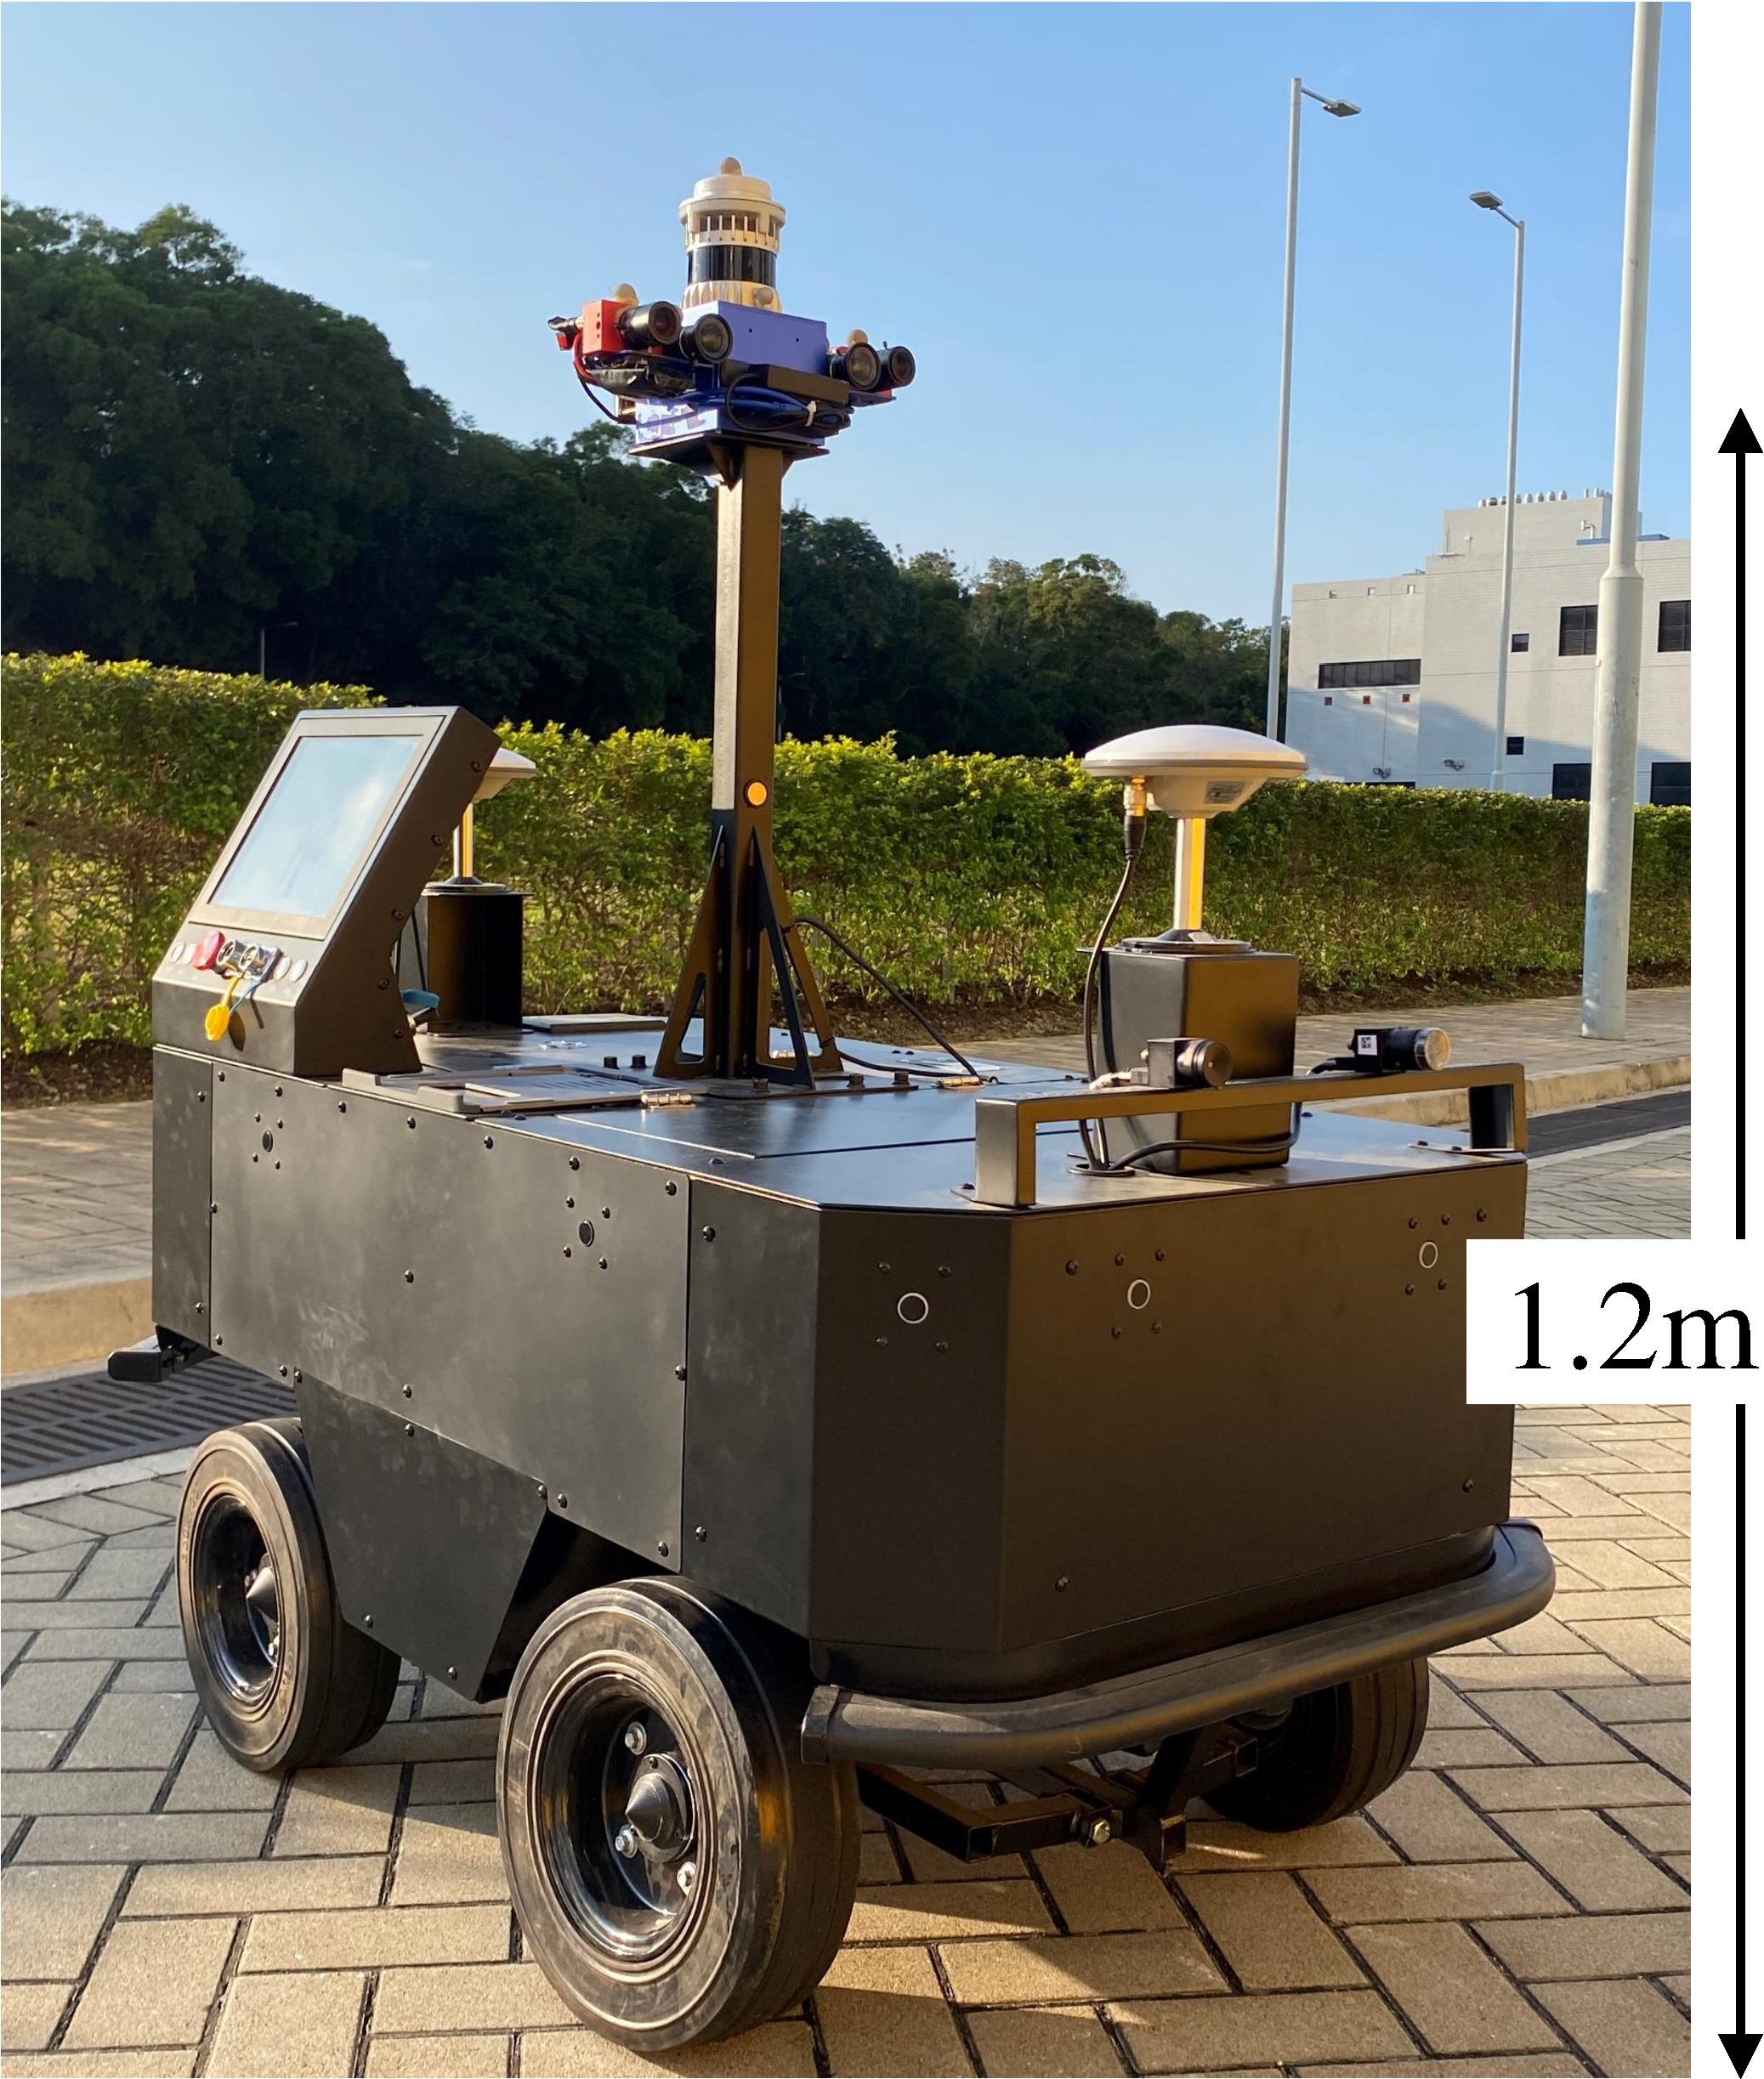
\includegraphics[width=.1701\linewidth]{figure/pqe/methodology/apollo-crop.pdf}} 
% \end{subfigure}
% \caption{The multi-sensor device and data collection platform: 
% (a) CAD model of the sensor rig, where axis directions are colored: red: $X$, green: $Y$, blue: $Z$. The sensor rig is rigidly mounted on (b) a gimbal stabilizer, (c) a quadruped robot, and (d) an apollo autonomous vehicle.}
% \label{fig:sensor_picture}
% \vspace{-0.3cm}
% \end{figure}  






% \showthe\font
%%%%%%%%%%%%%%%%%%%%%%%%%%%%%%%%%%%%%%%%%%%%%%%%%%%%%%%%%%%%%%%%%%%%%%%%%
%                                                                       %
%      9) BIBLIOGRAPHY                                                  %
%                                                                       %
% This example uses bibtex to generate the required Bibliography. Refer %
% to the % the file ustthesis_test.bib for the entries of the           %
% Bibliography. Note that only the cited entries are printed.           %
%                                                                       %
% If BibTeX is not used to typeset the bibliography, replace the        %
% following line with the \begin{thebibliography} and \end{bibliography}%
% commands (the "thebibliography" environment) to process the           %
% Bibliography.                                                         %
%                                                                       %
%%%%%%%%%%%%%%%%%%%%%%%%%%%%%%%%%%%%%%%%%%%%%%%%%%%%%%%%%%%%%%%%%%%%%%%%%

%%%%%%%%%%%%%%%%%%%%%%%%%%%%%%%%%%%%%%%%%%%%%%%%%%%%%%%%%%%%%%%%%%%%%%%%%
%                                                                       %
% The recommended bibliography style is the IEEE bibliography style.    %
% "ustbib" defines the IEEE bibliography standard with the added        %
% ability of sorting the items by name of author.                       %
%                                                                       %
% If you are not using BibTeX to process your Bibliography, comment out %
% the following line.                                                   %
%                                                                       %
%%%%%%%%%%%%%%%%%%%%%%%%%%%%%%%%%%%%%%%%%%%%%%%%%%%%%%%%%%%%%%%%%%%%%%%%%

\bibliographystyle{plain}

\bibliography{ref}

%%%%%%%%%%%%%%%%%%%%%%%%%%%%%%%%%%%%%%%%%%%%%%%%%%%%%%%%%%%%%%%%%%%%%%%%%
%                                                                       %
%     10) APPENDIX (If Any)                                             %
%                                                                       %
%                                                                       %
%%%%%%%%%%%%%%%%%%%%%%%%%%%%%%%%%%%%%%%%%%%%%%%%%%%%%%%%%%%%%%%%%%%%%%%%%



\end{document}
